\documentclass[12pt]{article}
\usepackage{amsmath, amssymb}
\usepackage{amsthm}
\usepackage{hyperref}
\usepackage{MnSymbol}
%%\usepackage[pdftex]{graphicx}
\usepackage{enumerate}
\usepackage{amsmath}
\usepackage{amssymb}
\usepackage{multicol}
\usepackage{algpseudocode}
\usepackage{algorithm}


\usepackage[final]{graphicx}
\usepackage{subcaption}
\renewcommand{\phi}{\varphi}
\newcommand{\rarrow}{\rightarrow}
\usepackage{ listings}
\title{COMP 576 Deep Learning}

\author{Guangyuan Yu(gy12)}


\begin{document}
\maketitle

\section{1 Backpropagation is a SNN}
\subsection{a Dataset}




\subsection{b.alpha-beta pruning}
10 leaves are visited. The cut off parts are in the block. Leaves with "x" are not visited. Nodes with "x" are not calculated.

\begin{figure}[H]
  \caption{center}
  \centering
    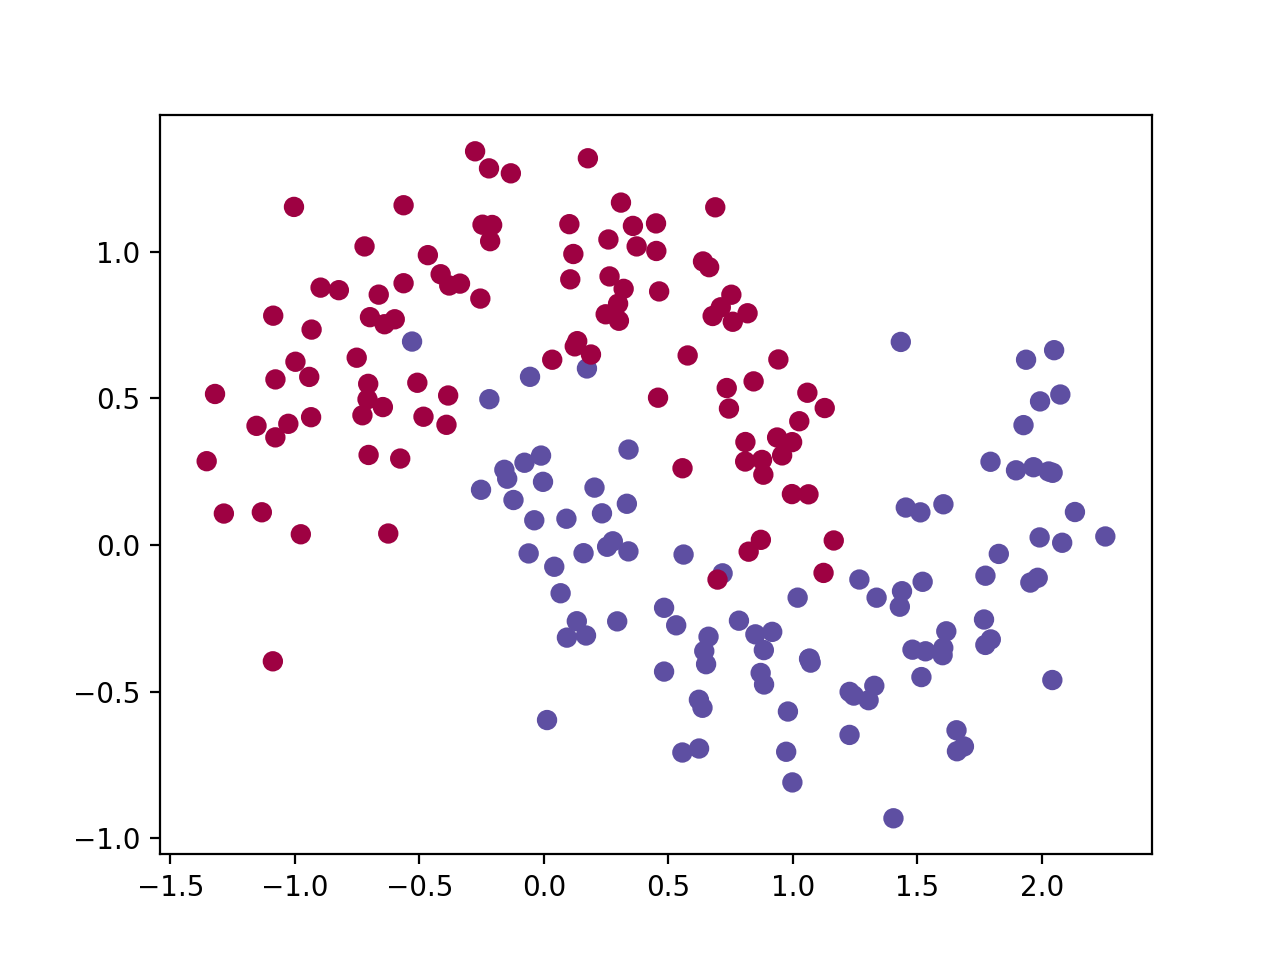
\includegraphics[scale=0.2]{figure1.png}
\end{figure}


\subsection{b.Activation Function}
1. 
\begin{lstlisting}

if type == 'tanh':
            value = np.tanh(z)
        elif type == 'sigmoid':
            value = 1 / (1 + np.exp(-z))
                   elif type == 'relu':
            
            value = z * (z > 0)
        else:
            raise Exception('Invalid activation function!')
\end{lstlisting}

\begin{figure}[H]
  \caption{center}
  \centering
    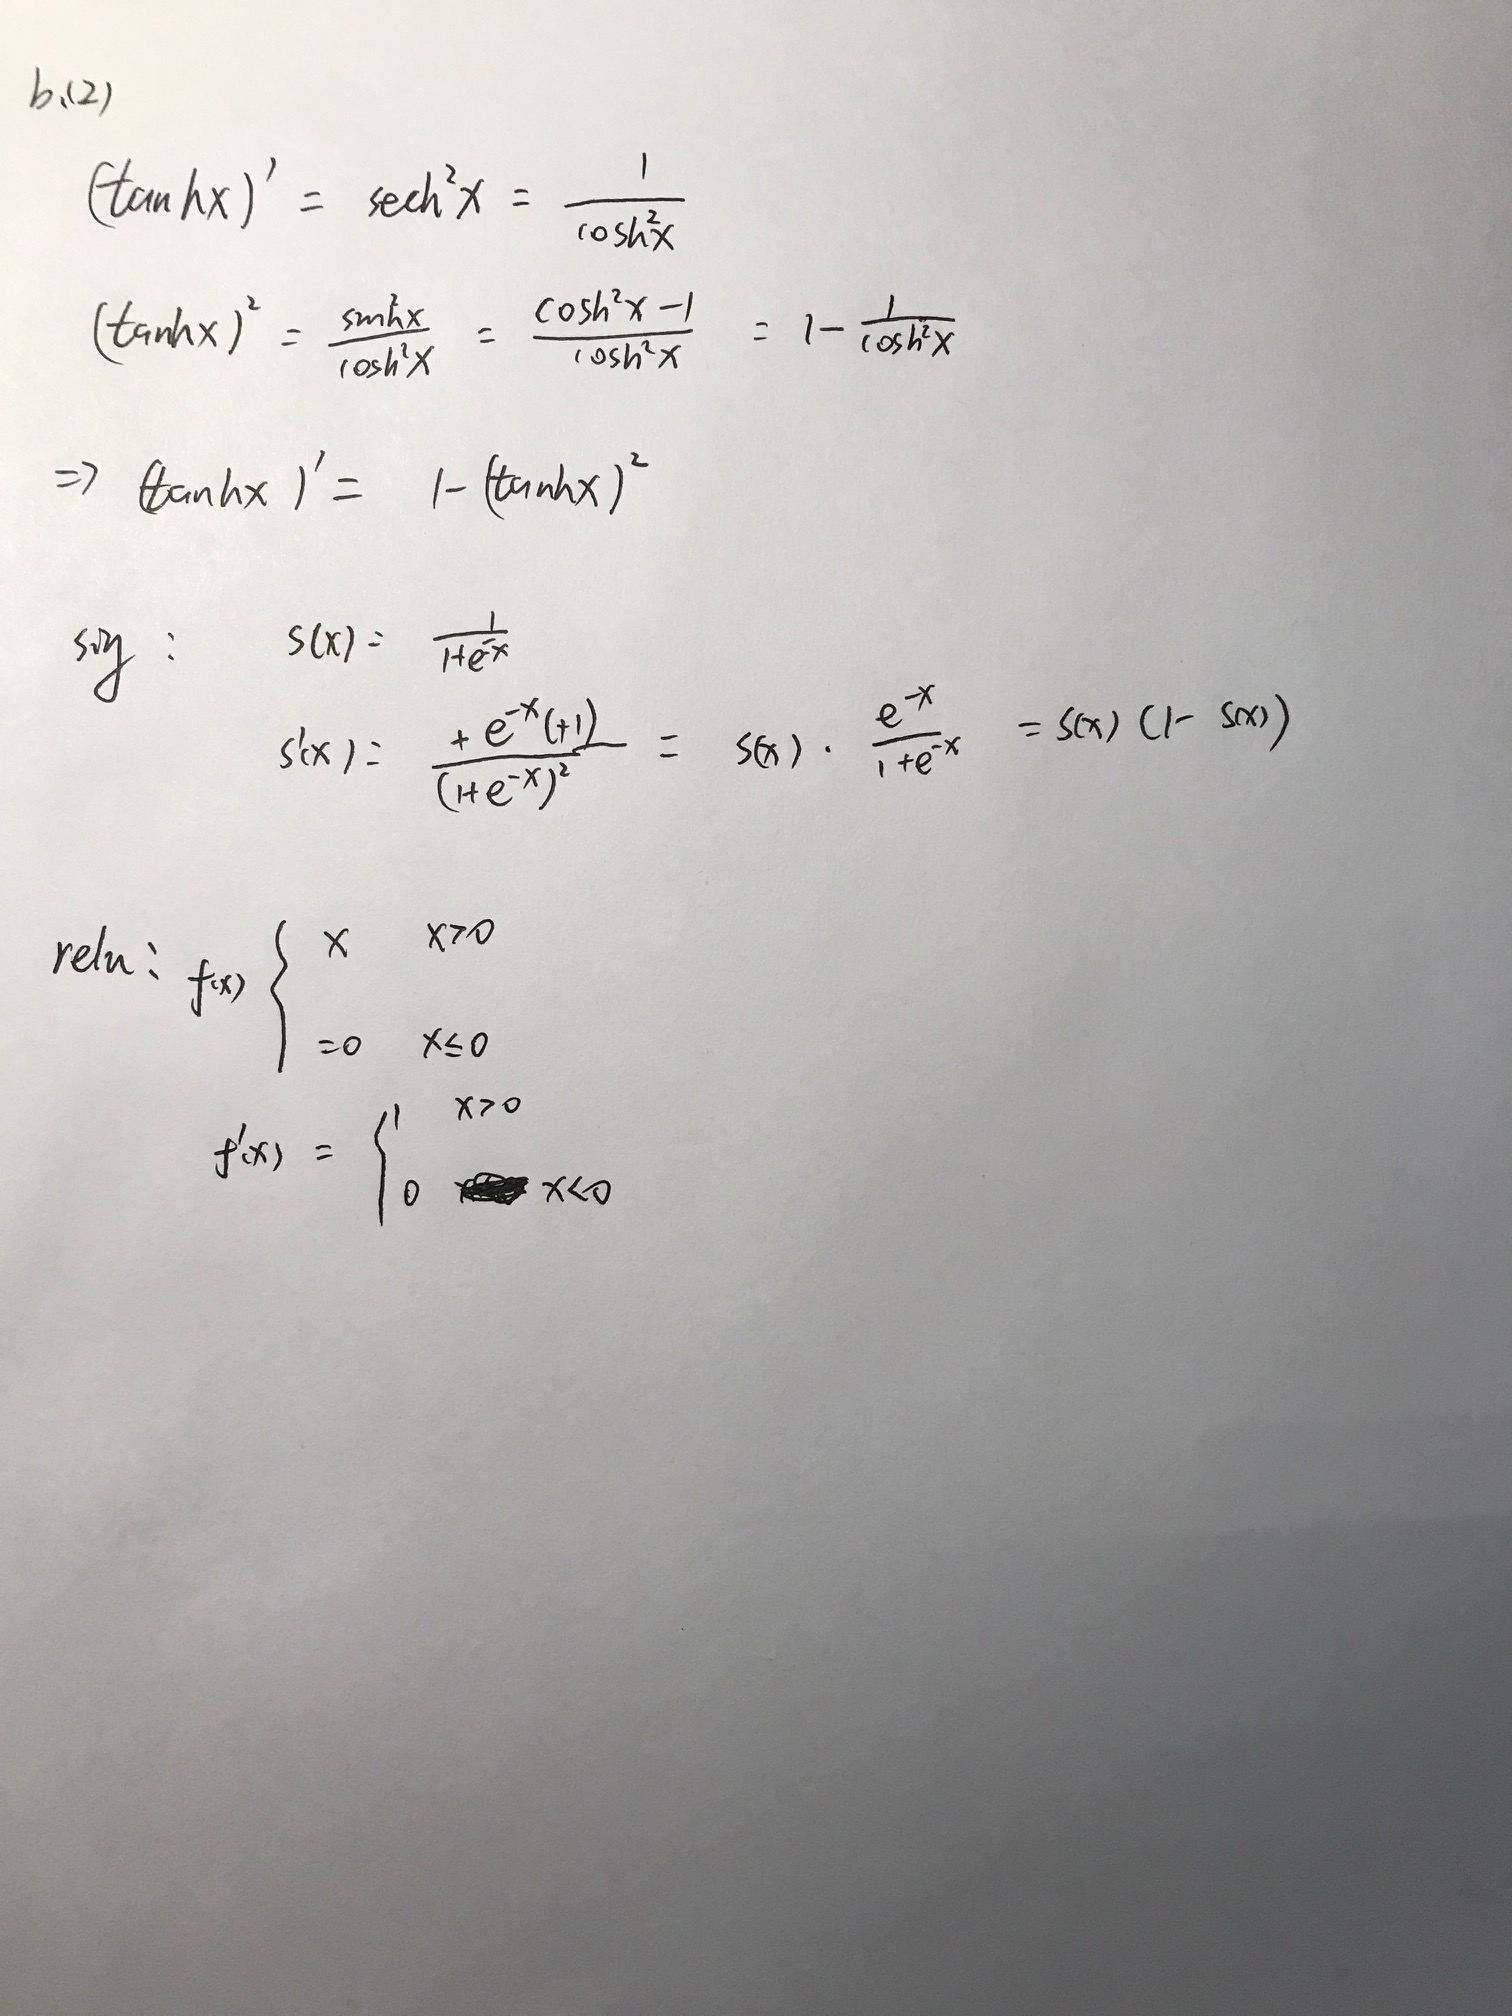
\includegraphics[scale=0.2]{b2.jpg}
\end{figure}
3.
\begin{lstlisting}
if type == 'tanh':
            value = np.tanh(z)
            diffvalue = 1 - (value * value)




        elif type == 'sigmoid':
            value = 1 / (1 + np.exp(-z))

            diffvalue = value * (1 - value)
        elif type == 'relu':
            
            diffvalue = (z > 0) * 1
\end{lstlisting}

\subsection{c}
1
\begin{lstlisting}
self.z1 = np.dot(X, self.W1) + self.b1
        self.a1 = actFun(self.z1)
        self.z2 = np.dot(self.a1, self.W2) + self.b2

        exp_scores = np.exp(self.z2)
        self.probs = exp_scores / np.sum(exp_scores, axis=1, keepdims=True)
\end{lstlisting}
2.
\begin{lstlisting}
data_loss = np.sum(-np.log(self.probs[range(num_examples), y]))
        # data_loss =


        data_loss += self.reg_lambda / 2 * (np.sum(np.square(self.W1)) + np.sum(np.square(self.W2)))
 \end{lstlisting}       



\subsection{d.}
1 
\begin{figure}[H]
  \caption{center}
  \centering
    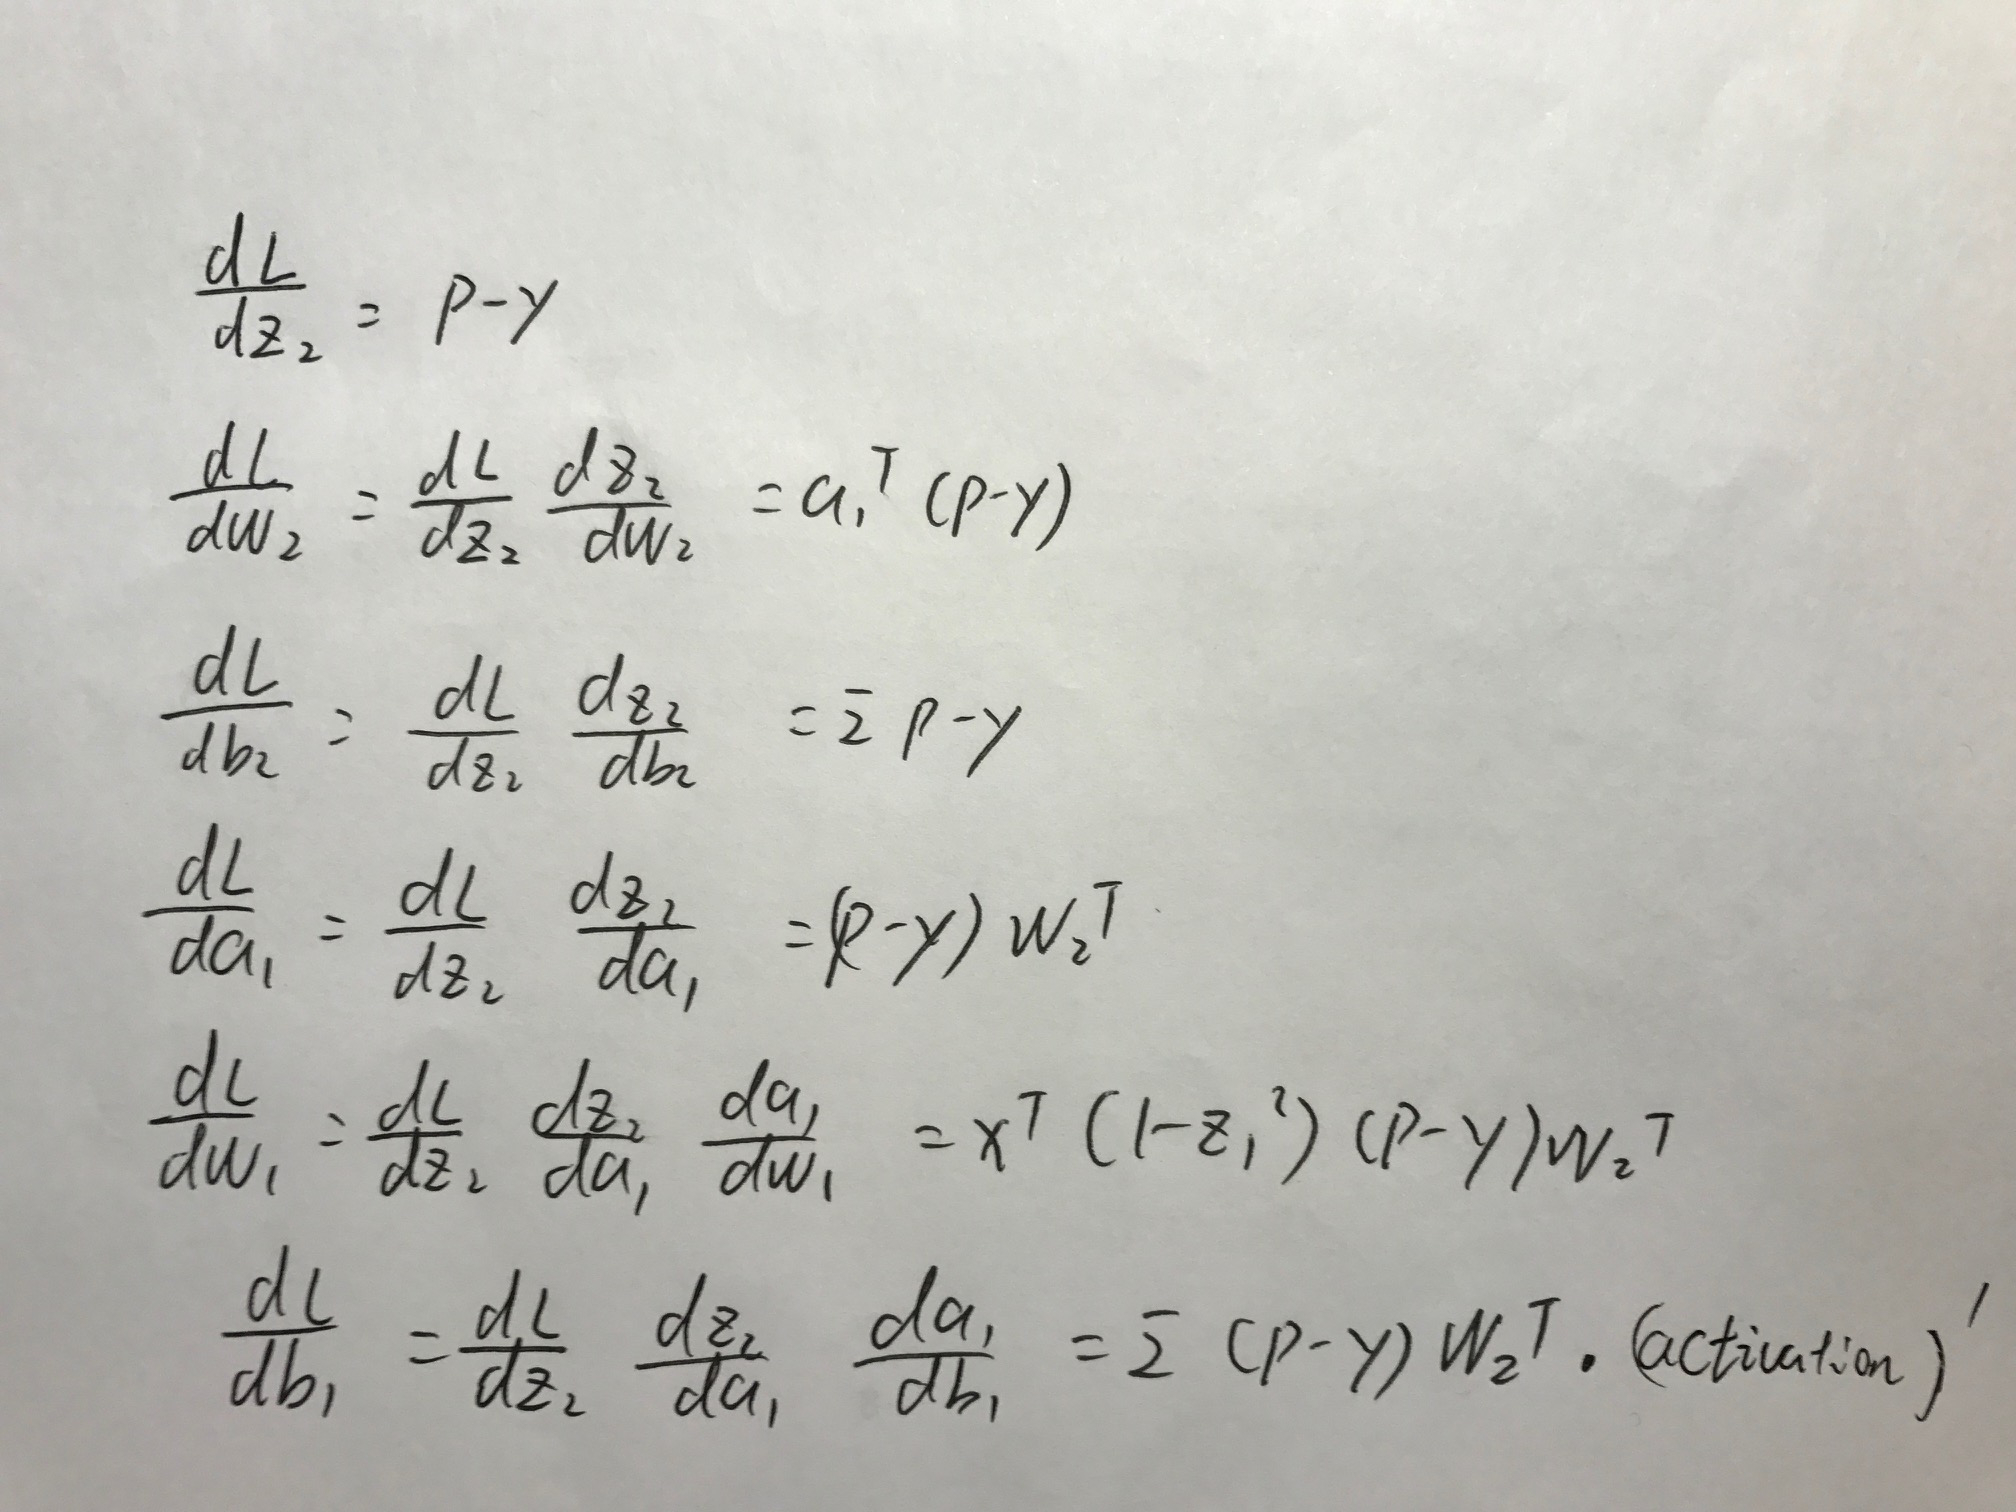
\includegraphics[scale=0.2]{b3.jpg}
\end{figure}
2
 \begin{lstlisting}  
num_examples = len(X)
        delta3 = self.probs
        delta3[range(num_examples), y] -= 1

        dW2 = (self.a1.T).dot(delta3)
        db2 = np.sum(delta3, axis=0, keepdims=True)
        delta2 = delta3.dot(self.W2.T) * self.diff_actFun(self.z1, self.actFun_type)
        dW1 = np.dot(X.T, delta2)
        db1 = np.sum(delta2, axis=0)
 \end{lstlisting}  
 
 

\subsection{e.}
1
\begin{figure}[H]
  \caption{center}
  \centering
    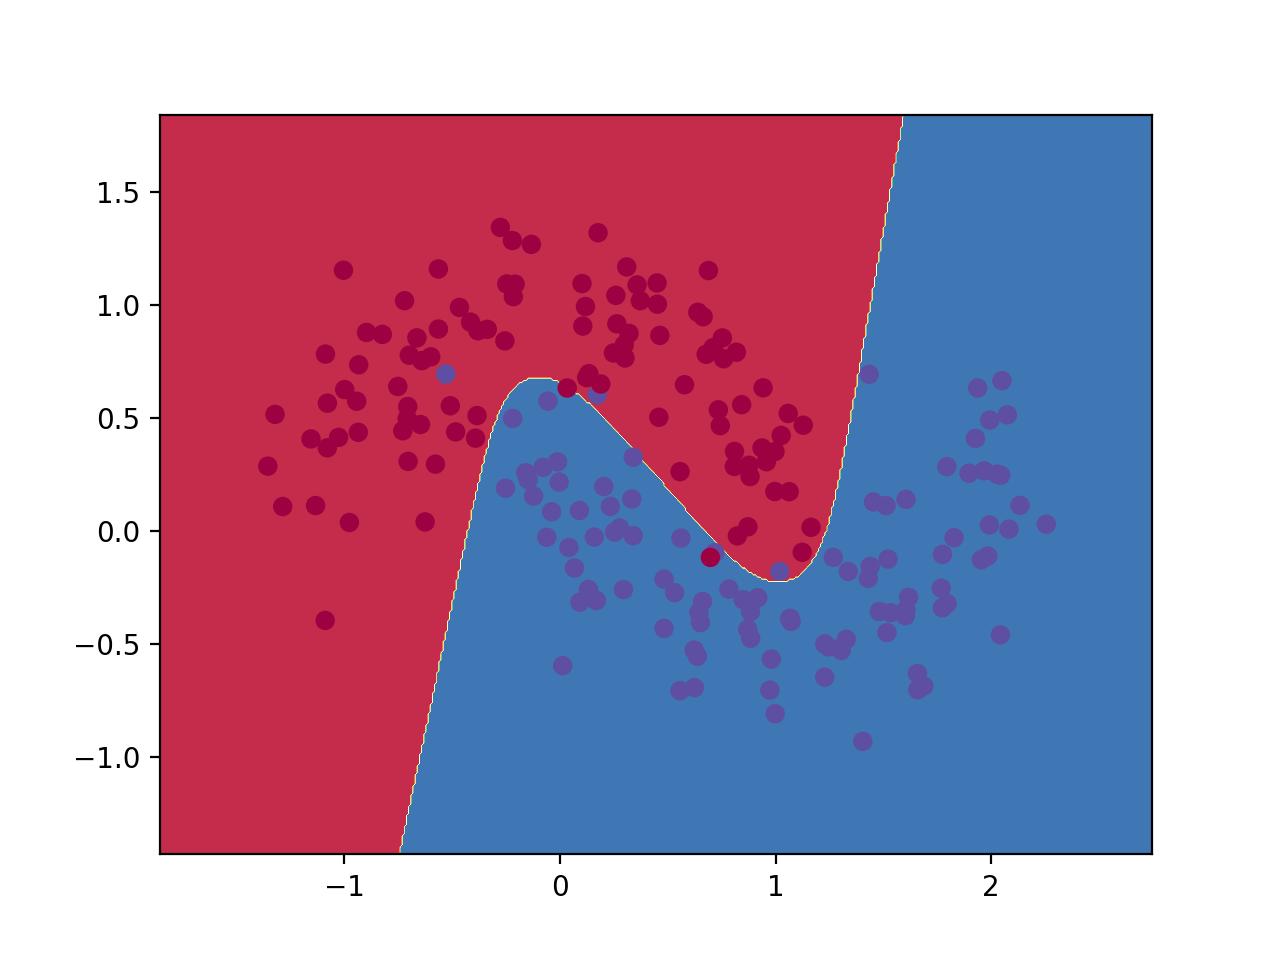
\includegraphics[scale=0.2]{tanh.png}
\end{figure}
\begin{figure}[H]
  \caption{center}
  \centering
    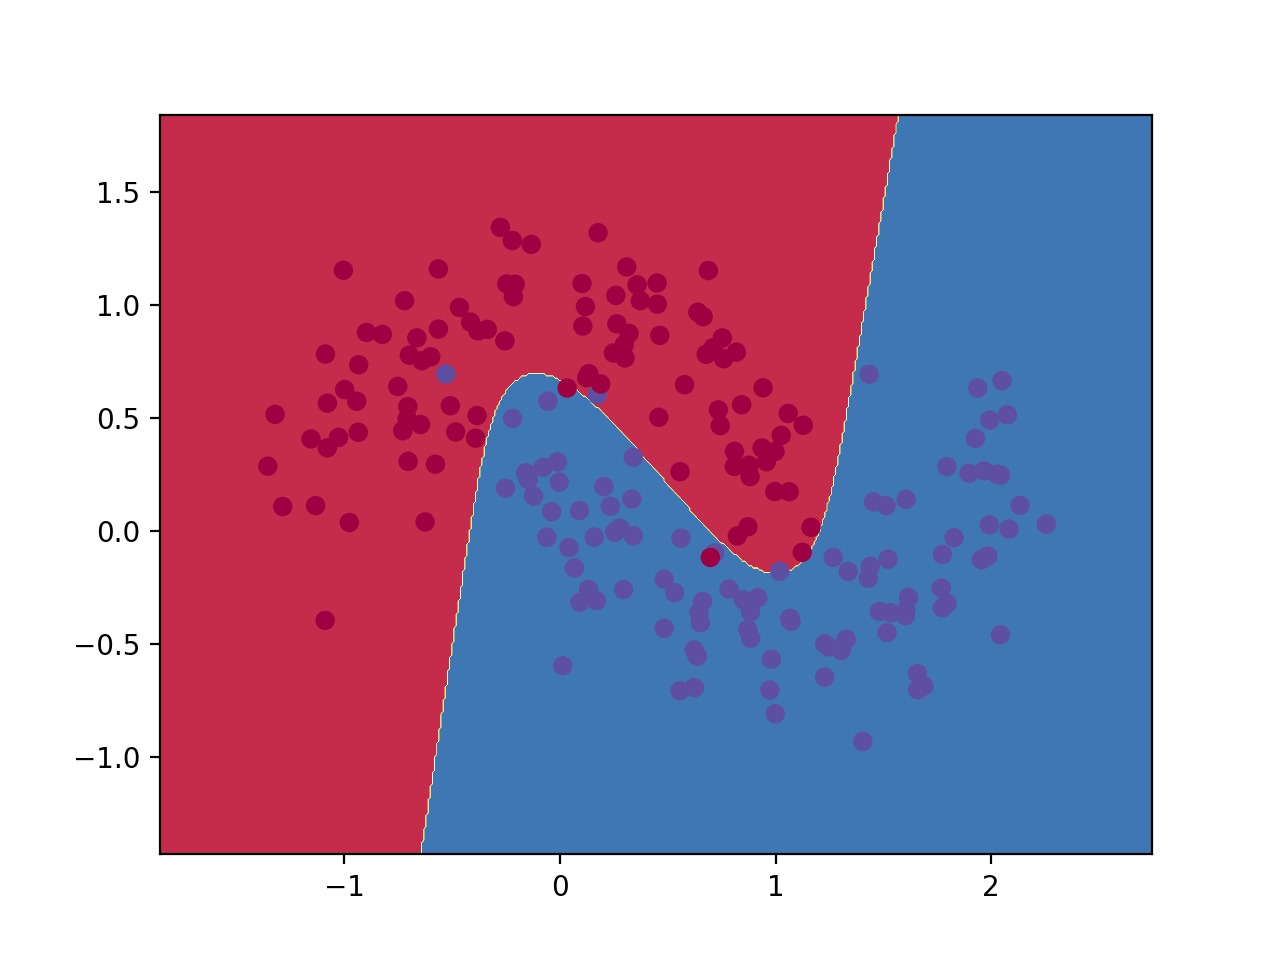
\includegraphics[scale=0.2]{sig.png}
\end{figure}
\begin{figure}[H]
  \caption{center}
  \centering
    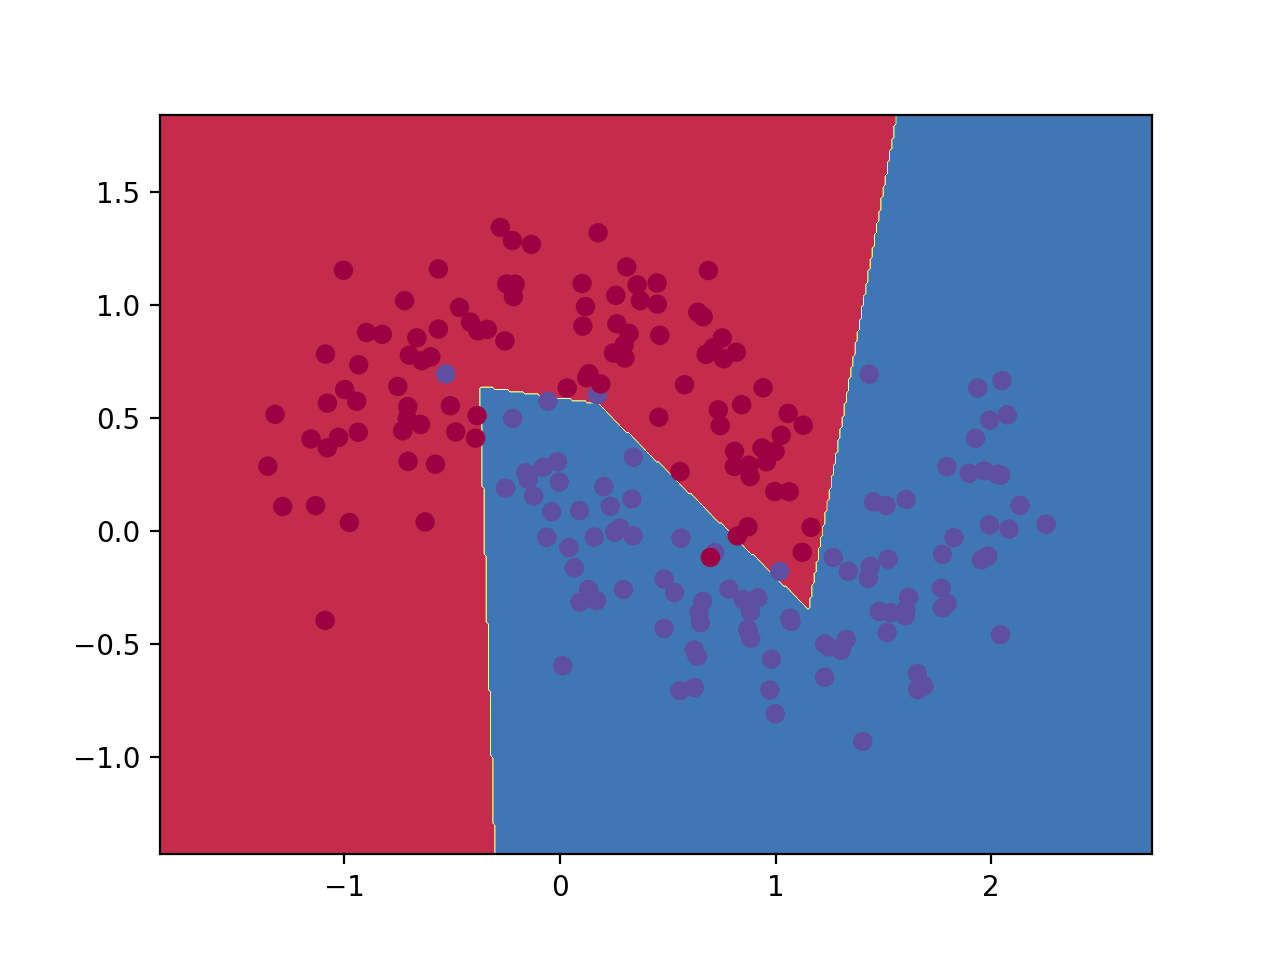
\includegraphics[scale=0.2]{relu.png}
\end{figure}

The decision boundary for sig and tanh are similar and smooth, while for relu, the boundary is very sharp.
This is because the relu function is not smooth. Some data point are not labeled correctly.
2

\begin{figure}[H]
  \caption{center}
  \centering
    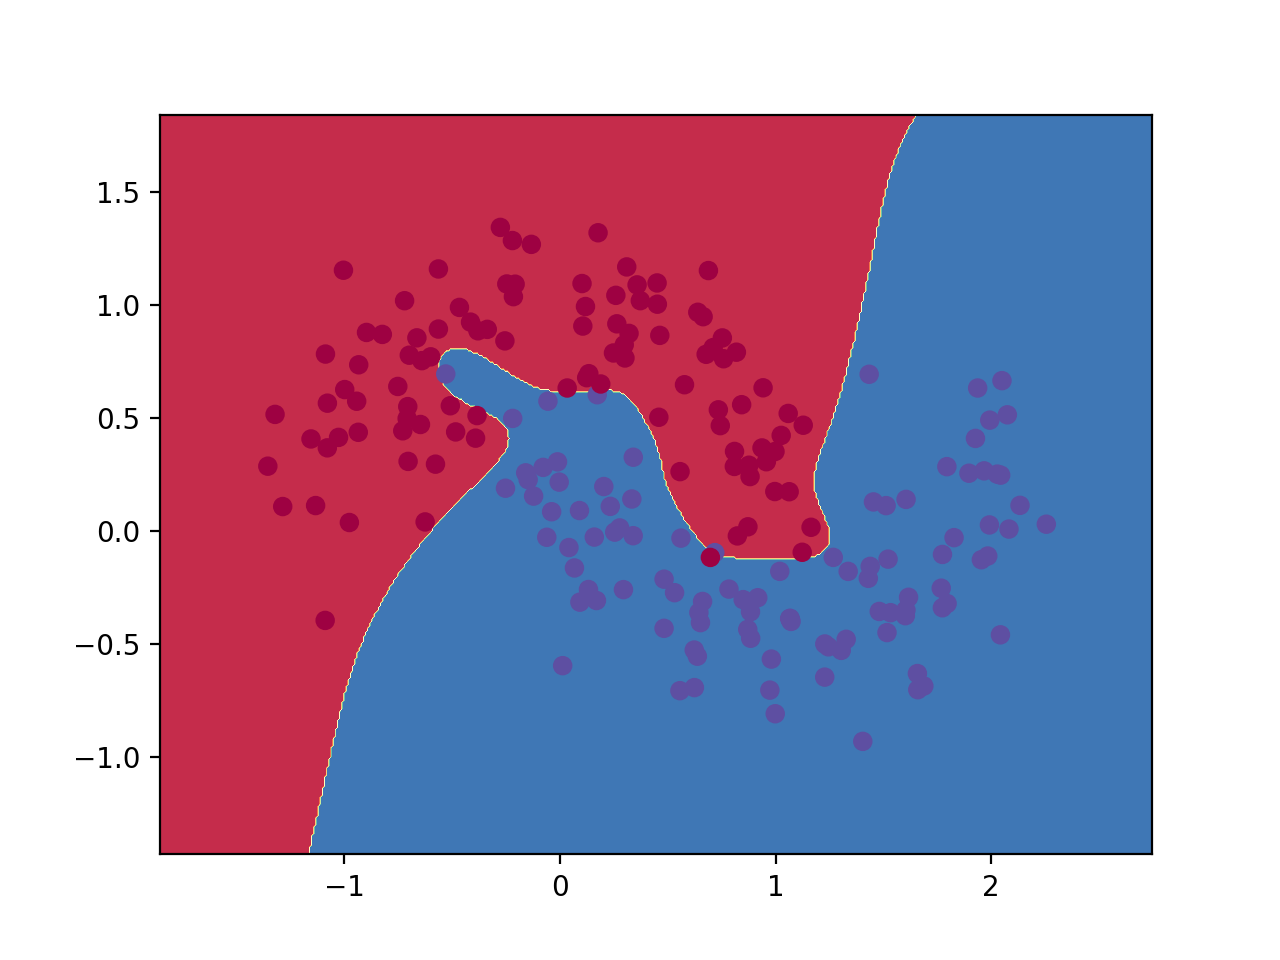
\includegraphics[scale=0.2]{10.png}
\end{figure}
Now I have 10 unit in hidden layers, The new plot is more curved and more data point are right labeled. It means increasing the hidden unit, the ability of the neurial network is increasing. 


\subsection{f.}
\begin{figure}[H]
  \caption{center}
  \centering
    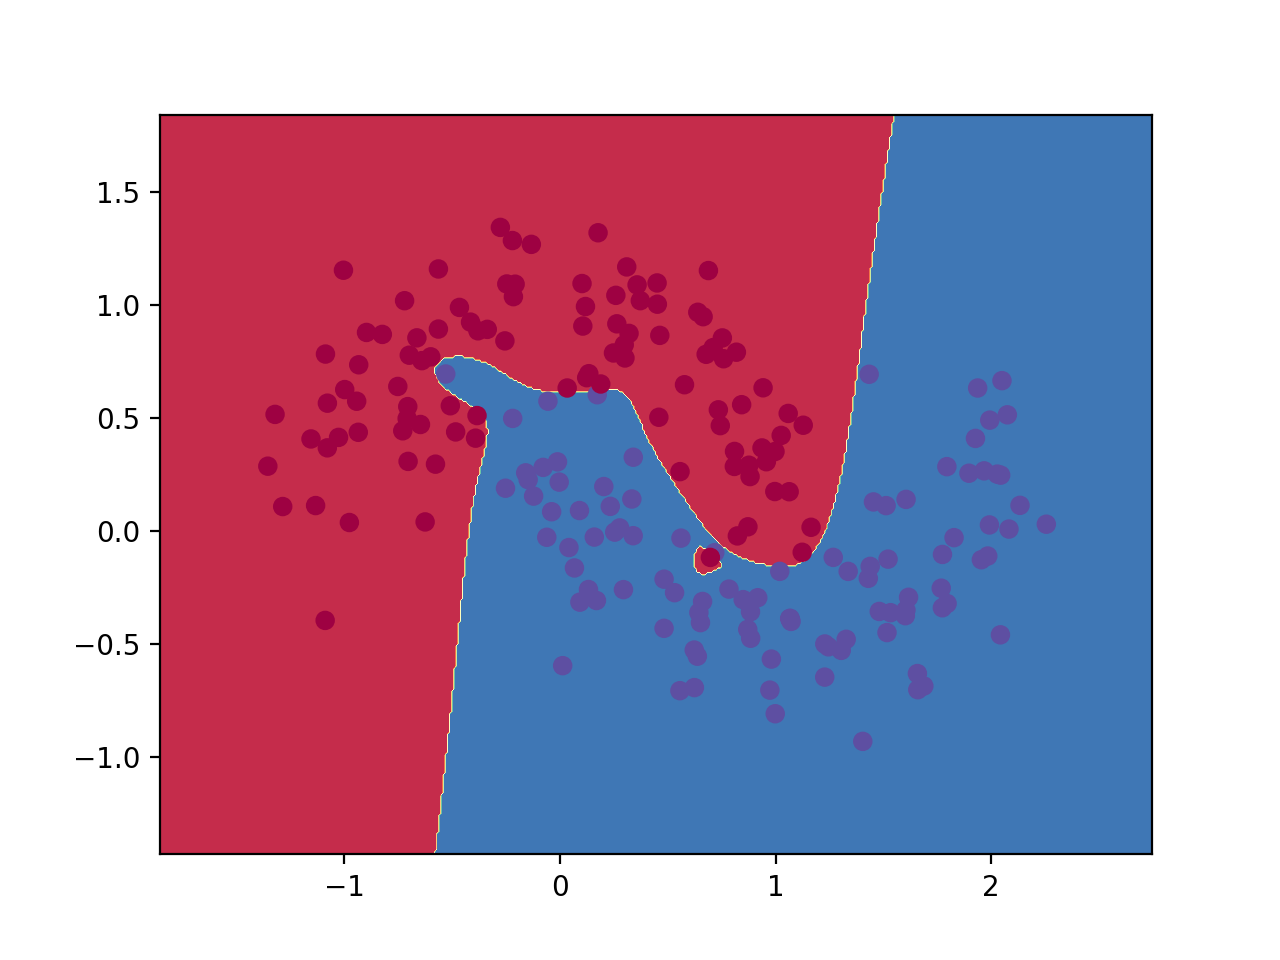
\includegraphics[scale=0.2]{6layer10tanh.png}
\end{figure}
It has 10 layers, and hidden layer have 6 units,relu.
\begin{figure}[H]
  \caption{center}
  \centering
    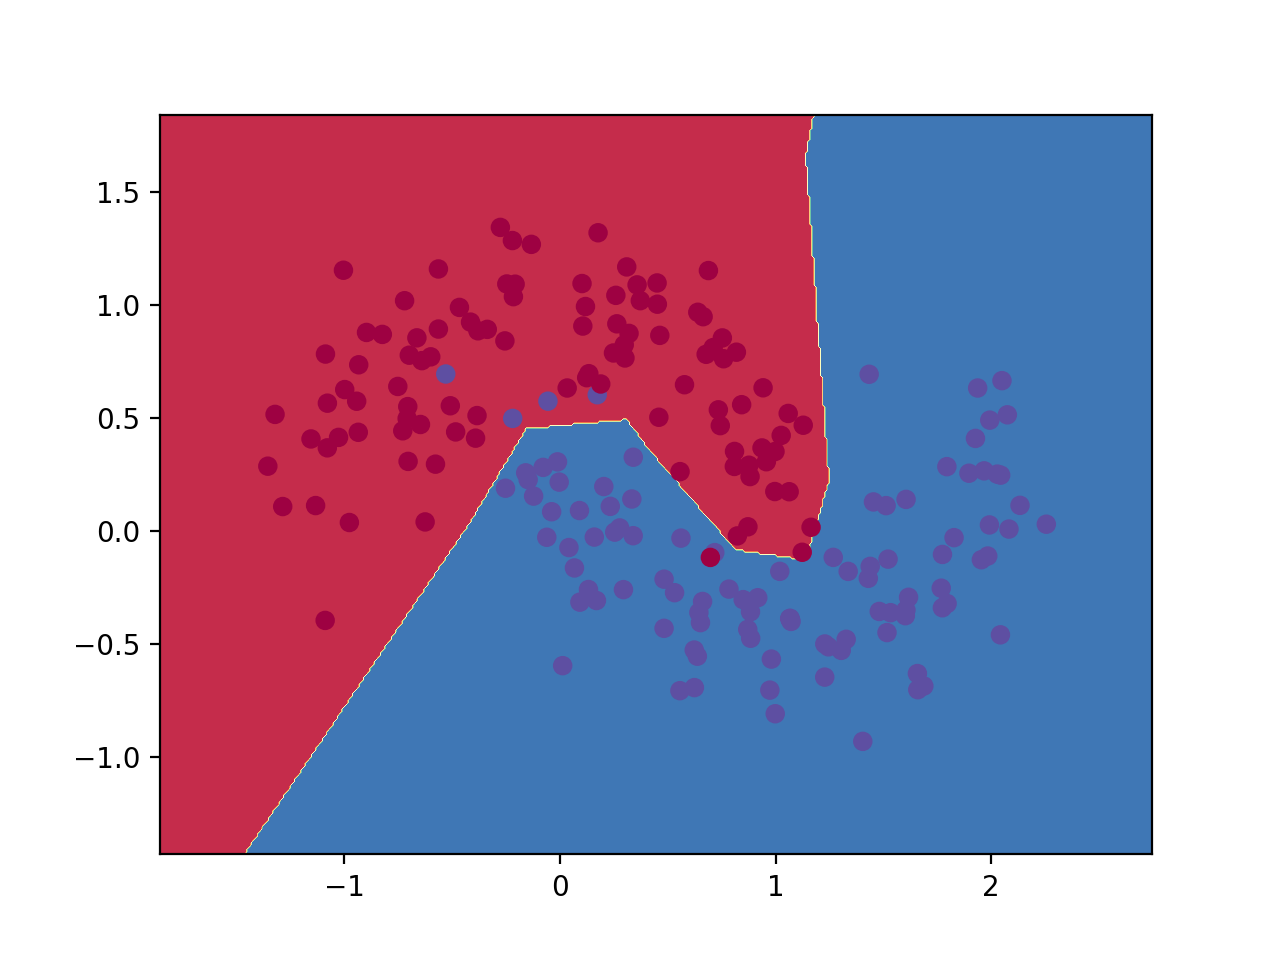
\includegraphics[scale=0.2]{6layer10relu.png}
\end{figure}
The decision boundary is slightly different from 10 layerthan, this one is more like a straight line. Since it is straight, there are more data point are not labeled correctly.



\begin{figure}[H]
  \caption{center}
  \centering
    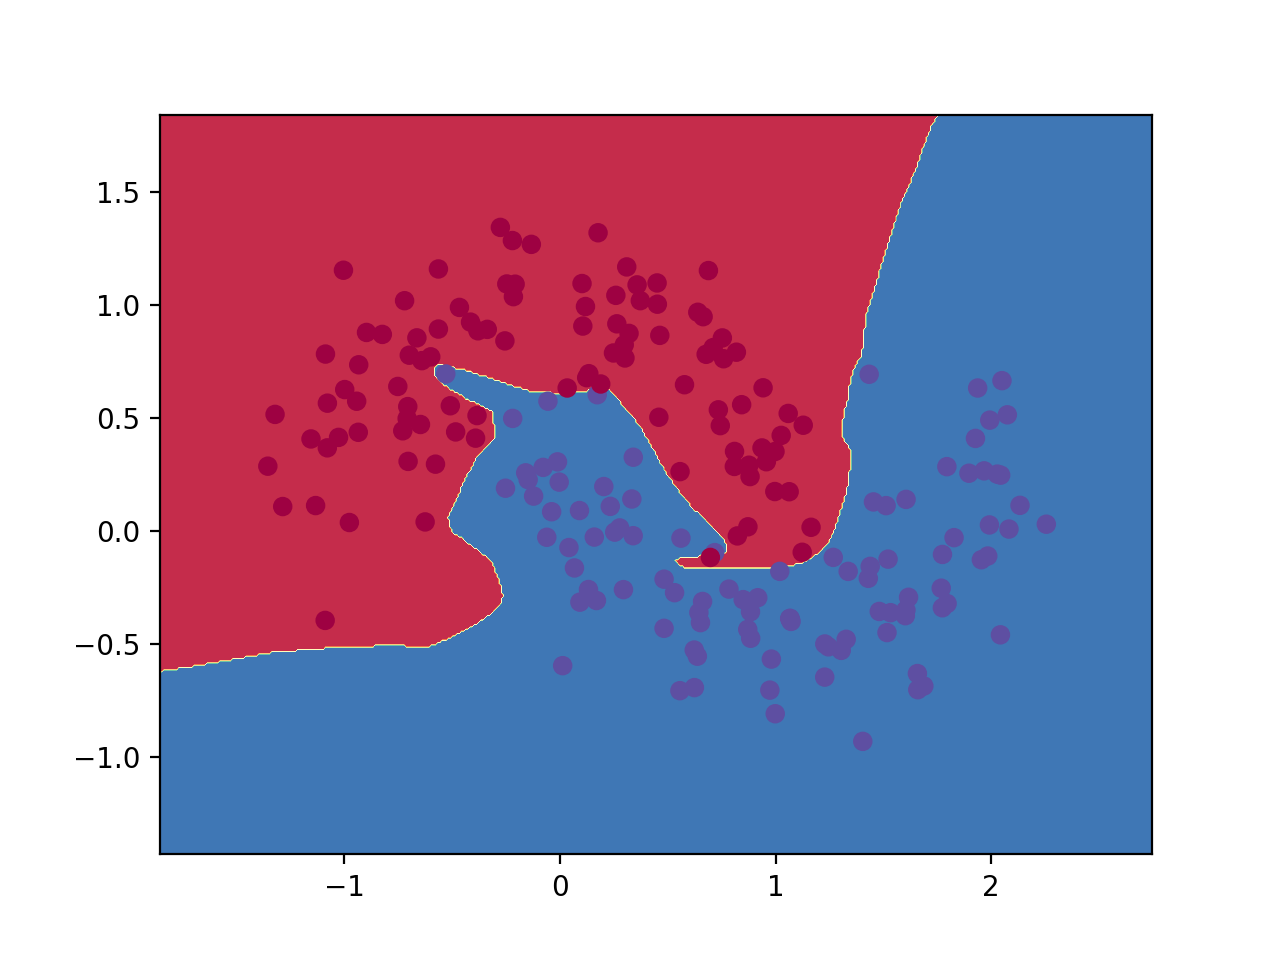
\includegraphics[scale=0.2]{20layer10relu.png}
\end{figure}
Then I used a 20 layer with 10 unit. now the relu could give a smooth boundary too.
\begin{figure}[H]
  \caption{center}
  \centering
    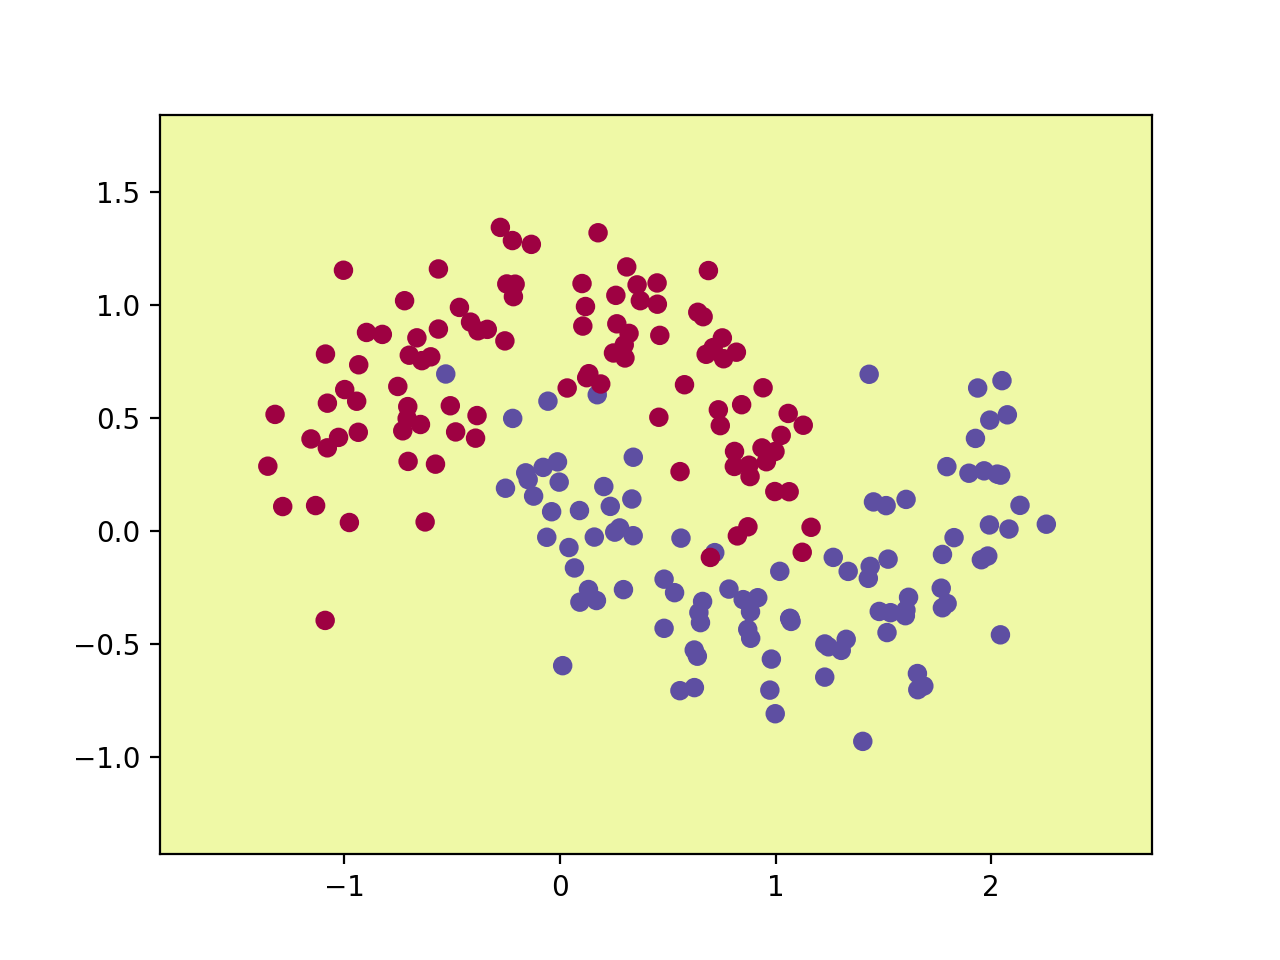
\includegraphics[scale=0.2]{deep.png}
\end{figure}
When it is too deep, the loss would not change, it is alway around 0.7. It is because the relu could not pass the gradient back. it is dead relu.
\begin{figure}[H]
  \caption{center}
  \centering
    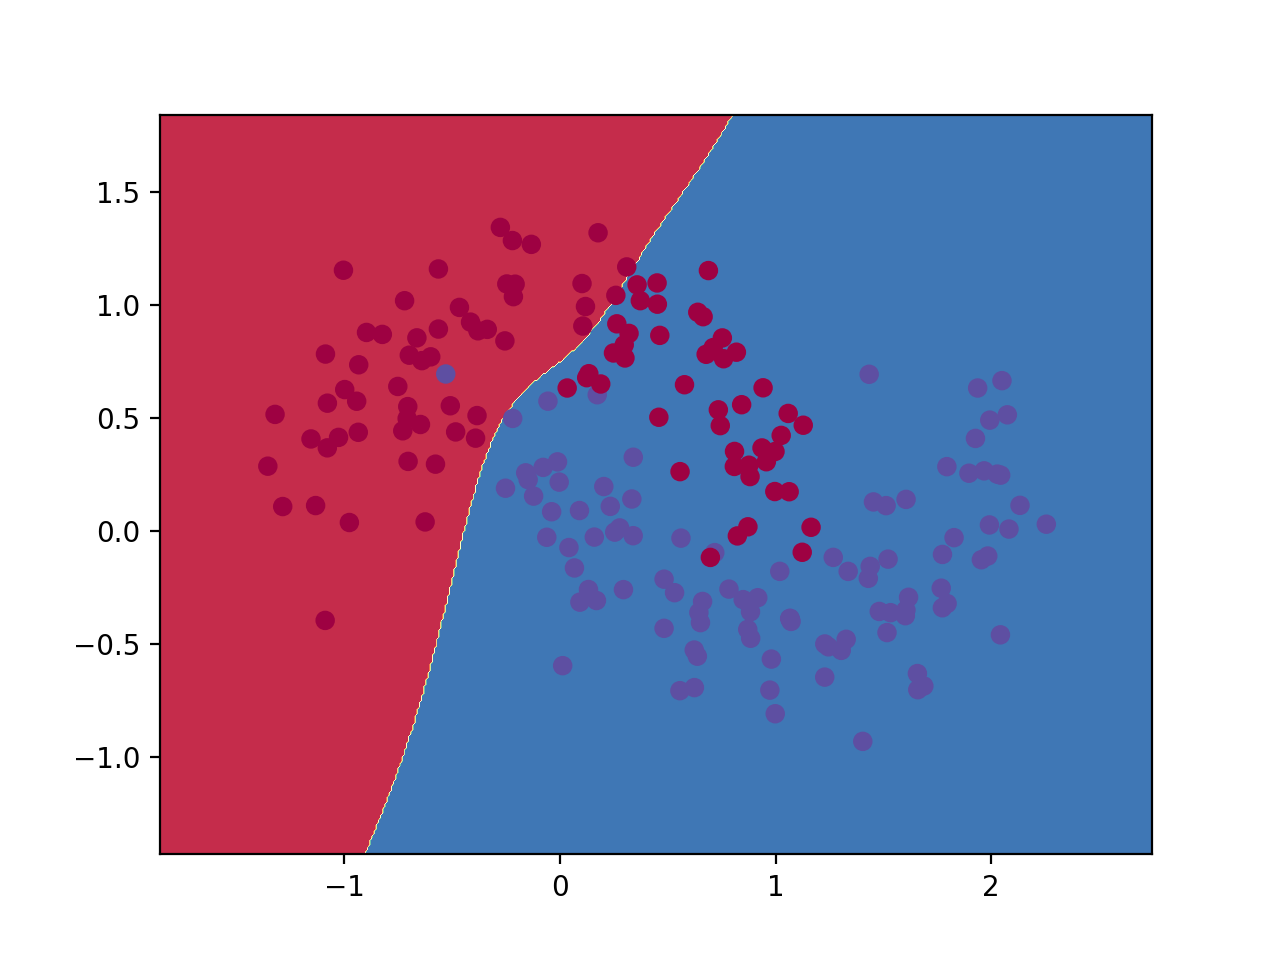
\includegraphics[scale=0.2]{tandeep.png}
\end{figure}
The same structure for tanh function, the problem will be overfitting. the loss goes to 0.06 then ,finally go to 0.5. But, tanh can back propagate. Since the gradient of tanh is not flat, it alwasy works.  


\subsection{On another dataset}
\begin{figure}[H]
  \caption{center}
  \centering
    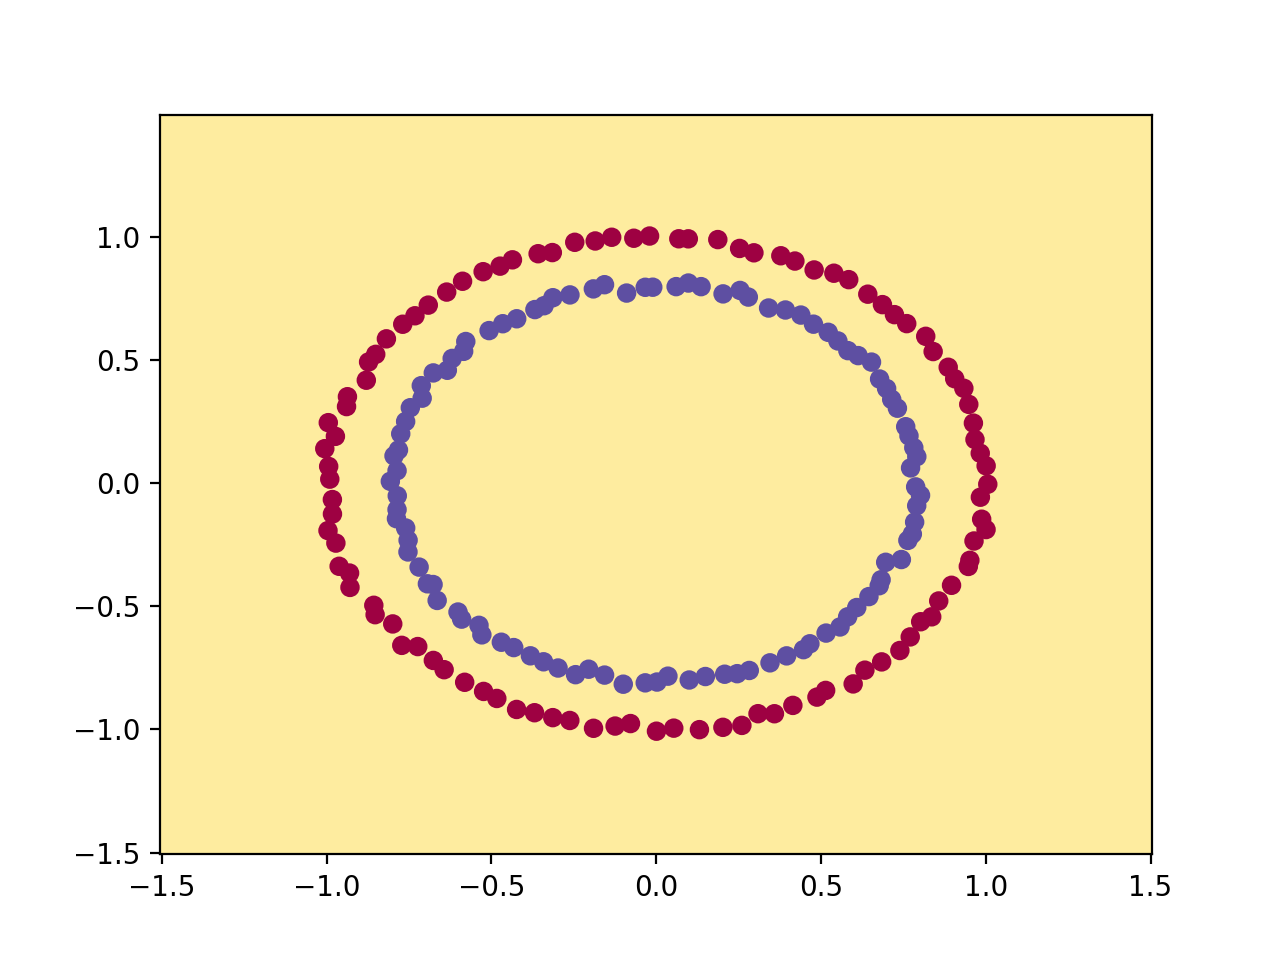
\includegraphics[scale=0.2]{tandead.png}
\end{figure}
On this dataset, tanh also dead on deep network. 30 layers. 30 unit.
Relu also dead here.
\begin{figure}[H]
  \caption{center}
  \centering
    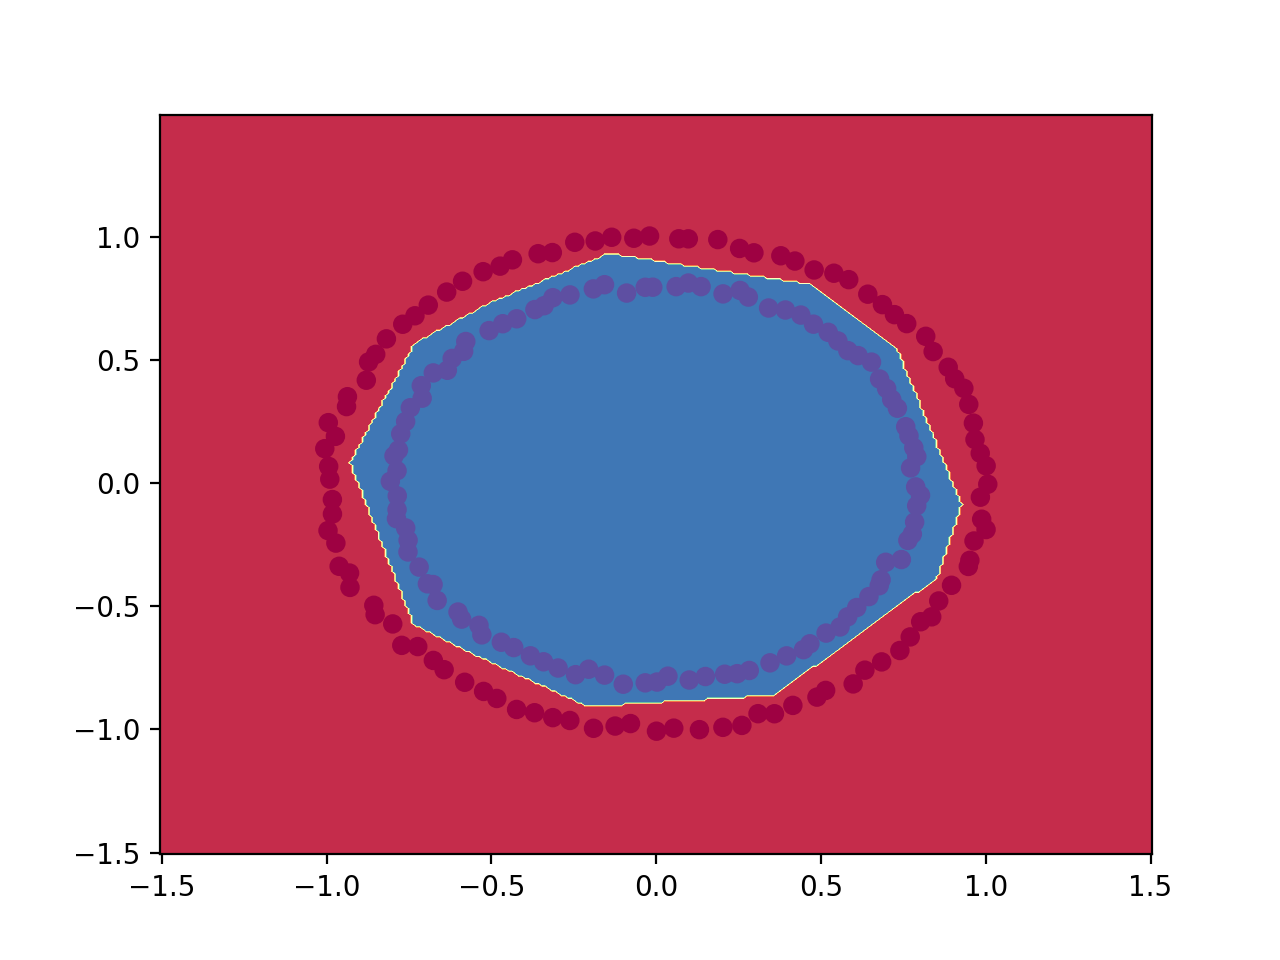
\includegraphics[scale=0.2]{4layer6relu.png}
\end{figure}
This is a relu with 4 layer, 4 unit. The boundary is not smooth. 
\begin{figure}[H]
  \caption{center}
  \centering
    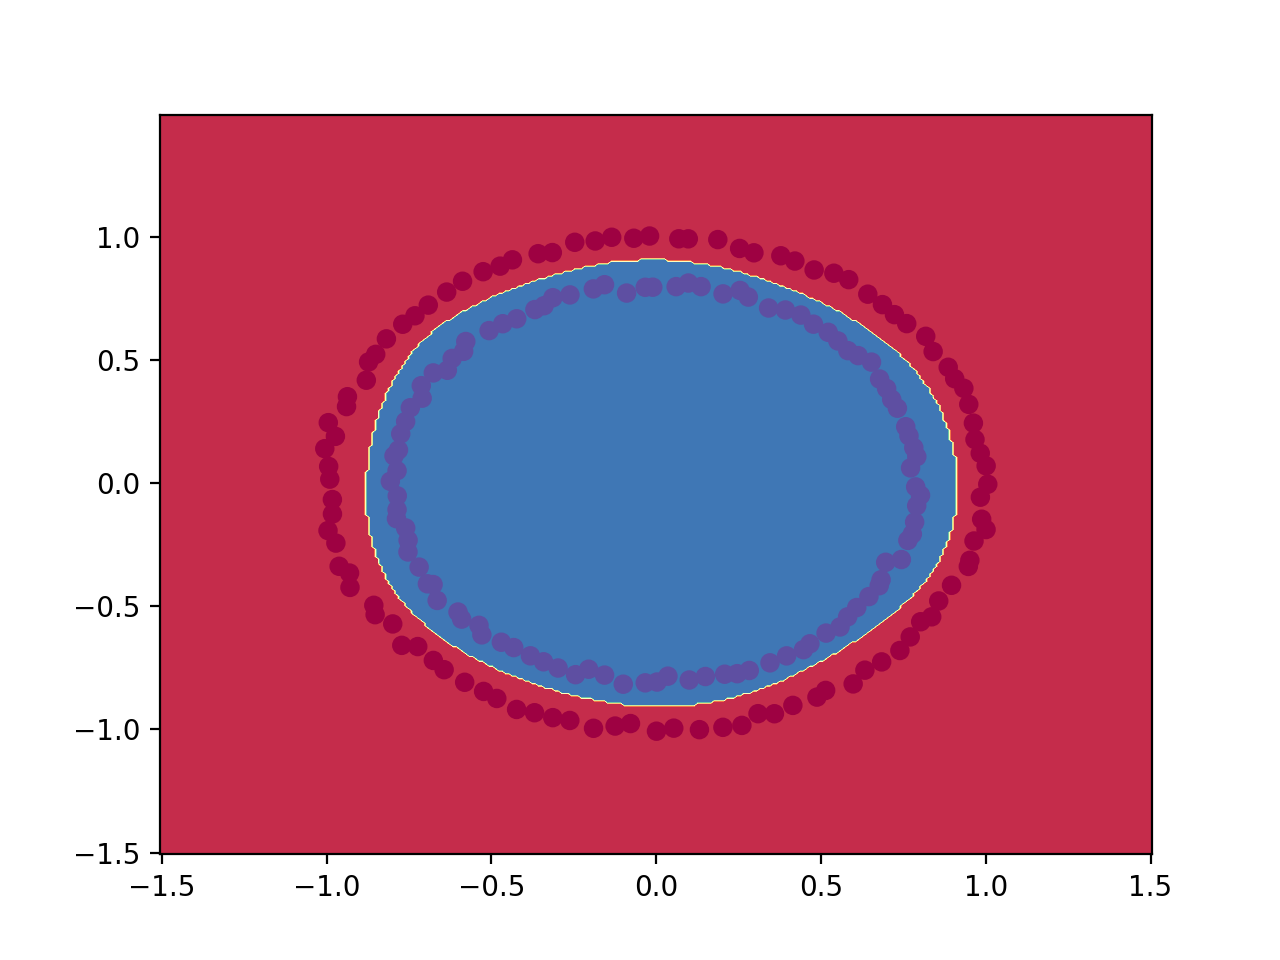
\includegraphics[scale=0.2]{4layer6tanh.png}
\end{figure}
This is tanh, the boundry is smooth.






\section{Training a simple DCN on MNIST}
\subsection{A}
SEE THE CODE FILE
(5)
admin relu
step 5400, training accuracy 0.98
step 5500, training accuracy 1
test accuracy 0.988
The training takes 53.495326 second to finish
(6)
\begin{figure}[H]
  \caption{center}
  \centering
    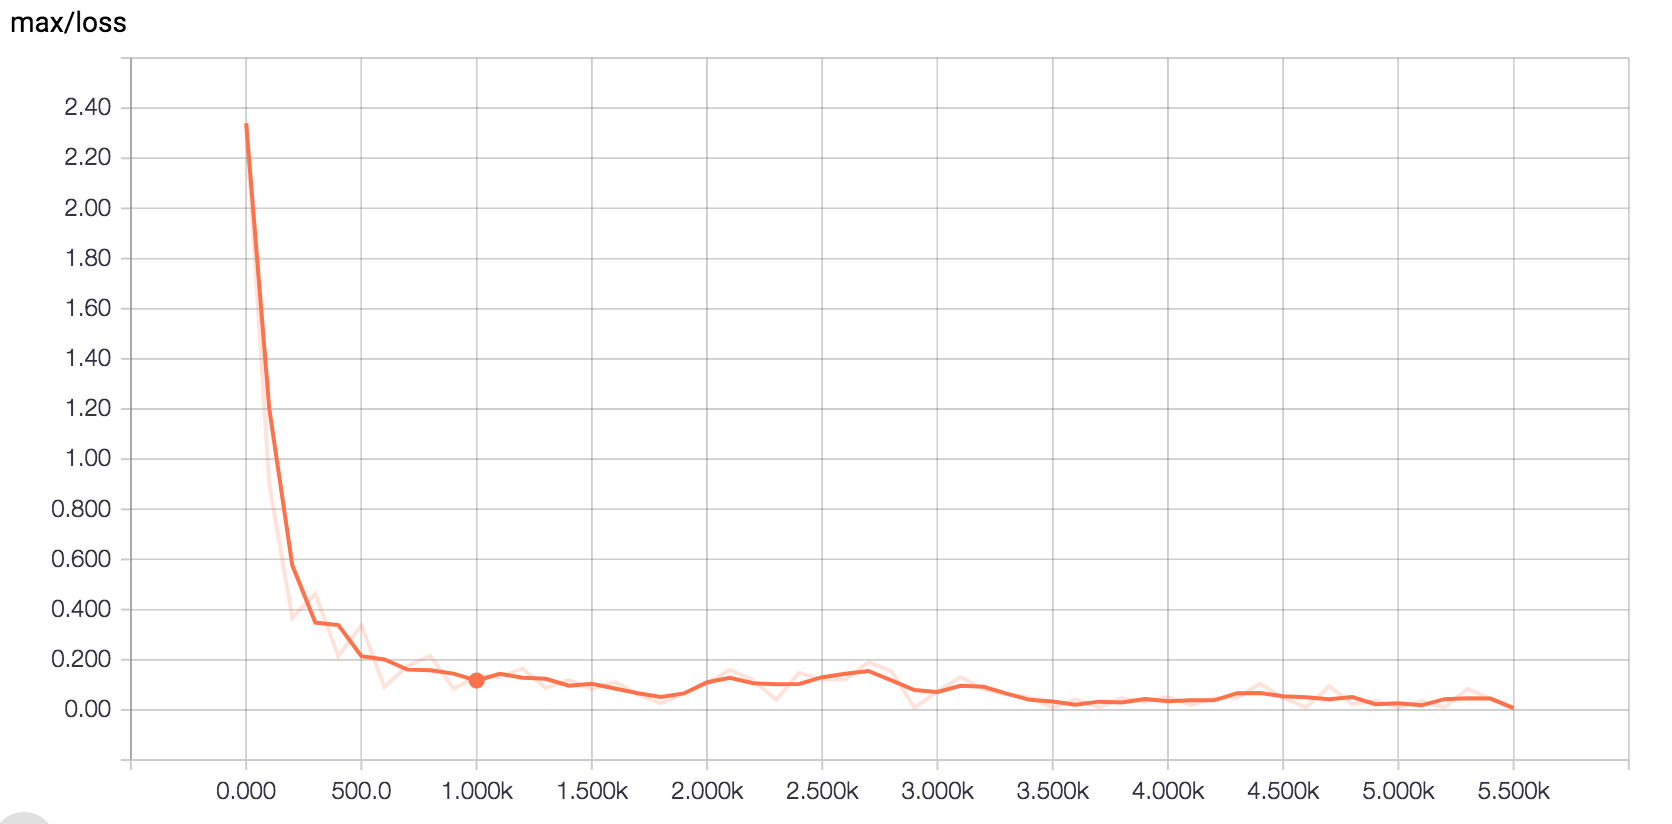
\includegraphics[scale=0.4]{6lossmax.png}
\end{figure}



\subsection{B}
\begin{figure}[H]
  \caption{center}
  \centering
    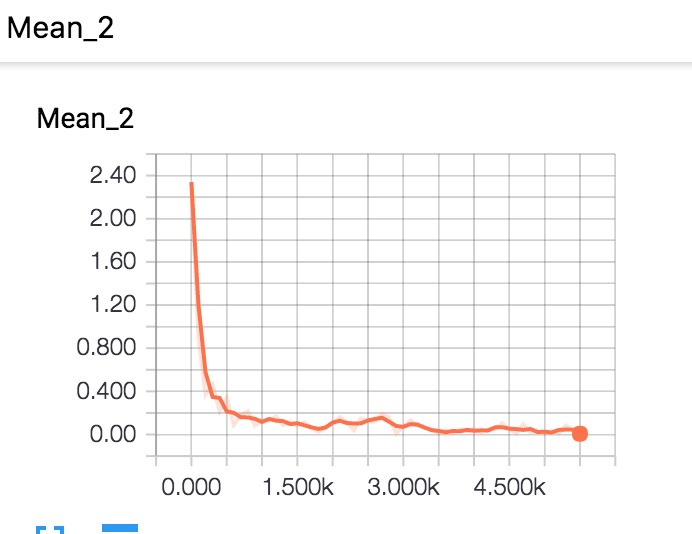
\includegraphics[scale=0.3]{bmean.png}
\end{figure}






\begin{figure}[H]
  \caption{center}
  \centering
    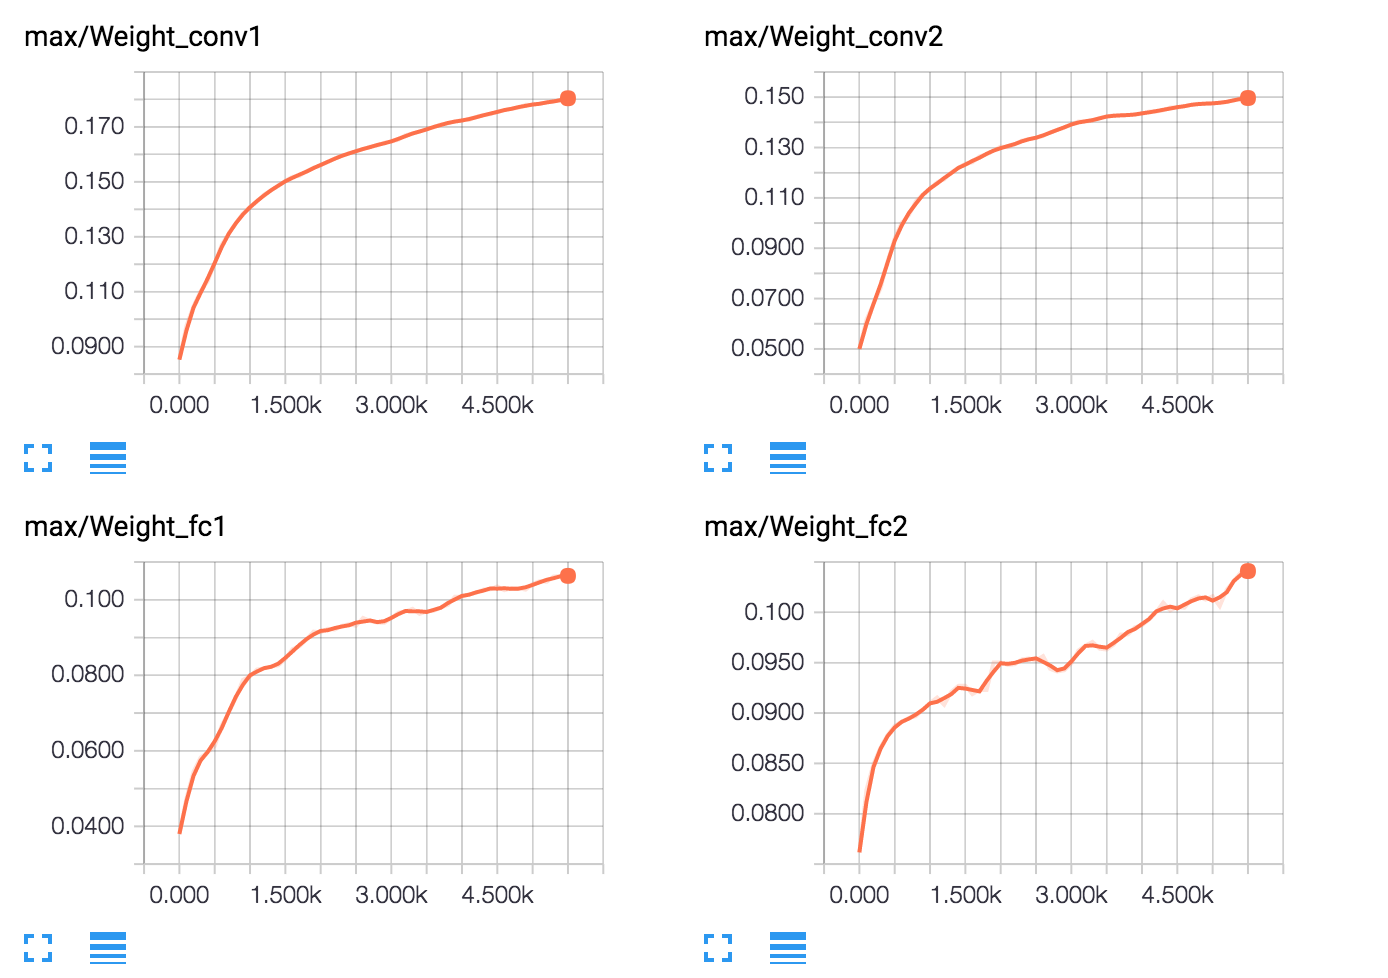
\includegraphics[scale=0.3]{bmax1.png}
\end{figure}
\begin{figure}[H]
  \caption{center}
  \centering
    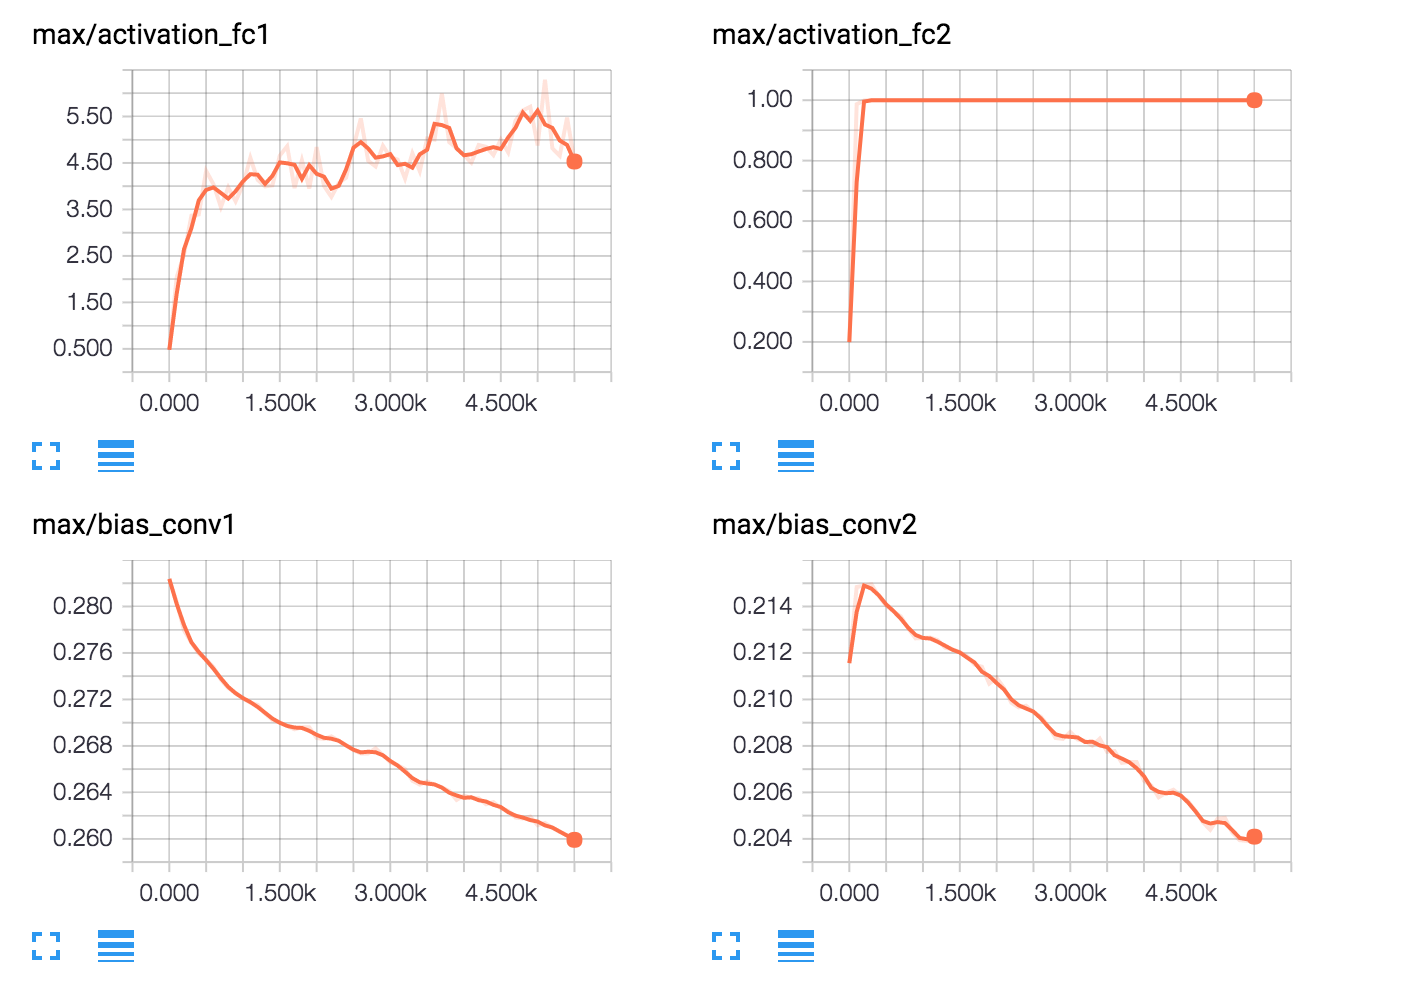
\includegraphics[scale=0.3]{bmax2.png}
\end{figure}

\begin{figure}[H]
  \caption{center}
  \centering
    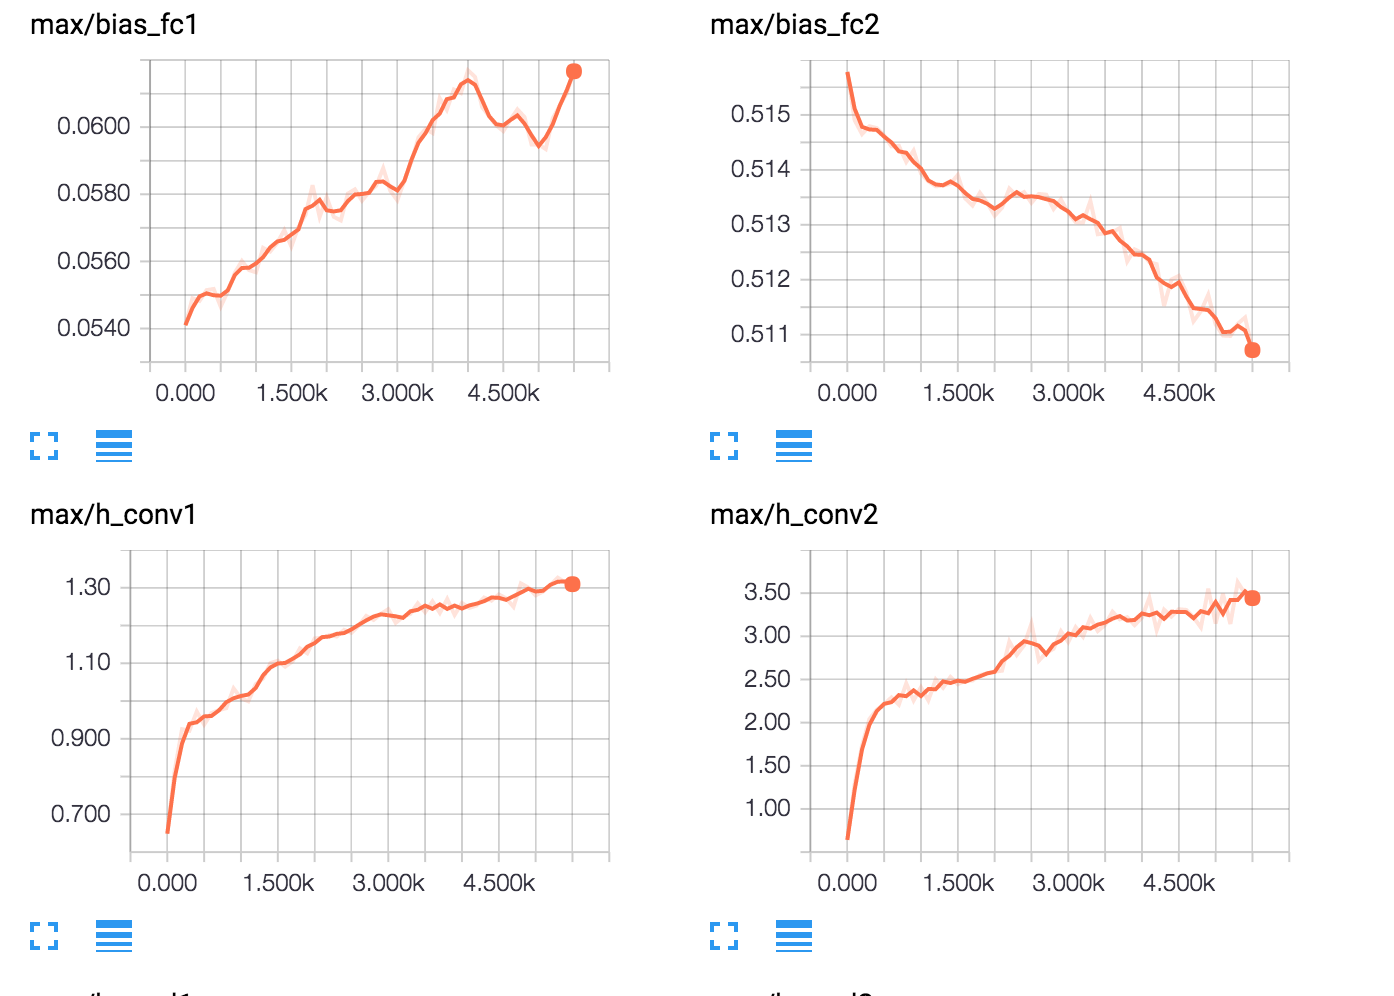
\includegraphics[scale=0.3]{bmax3.png}
\end{figure}

\begin{figure}[H]
  \caption{center}
  \centering
    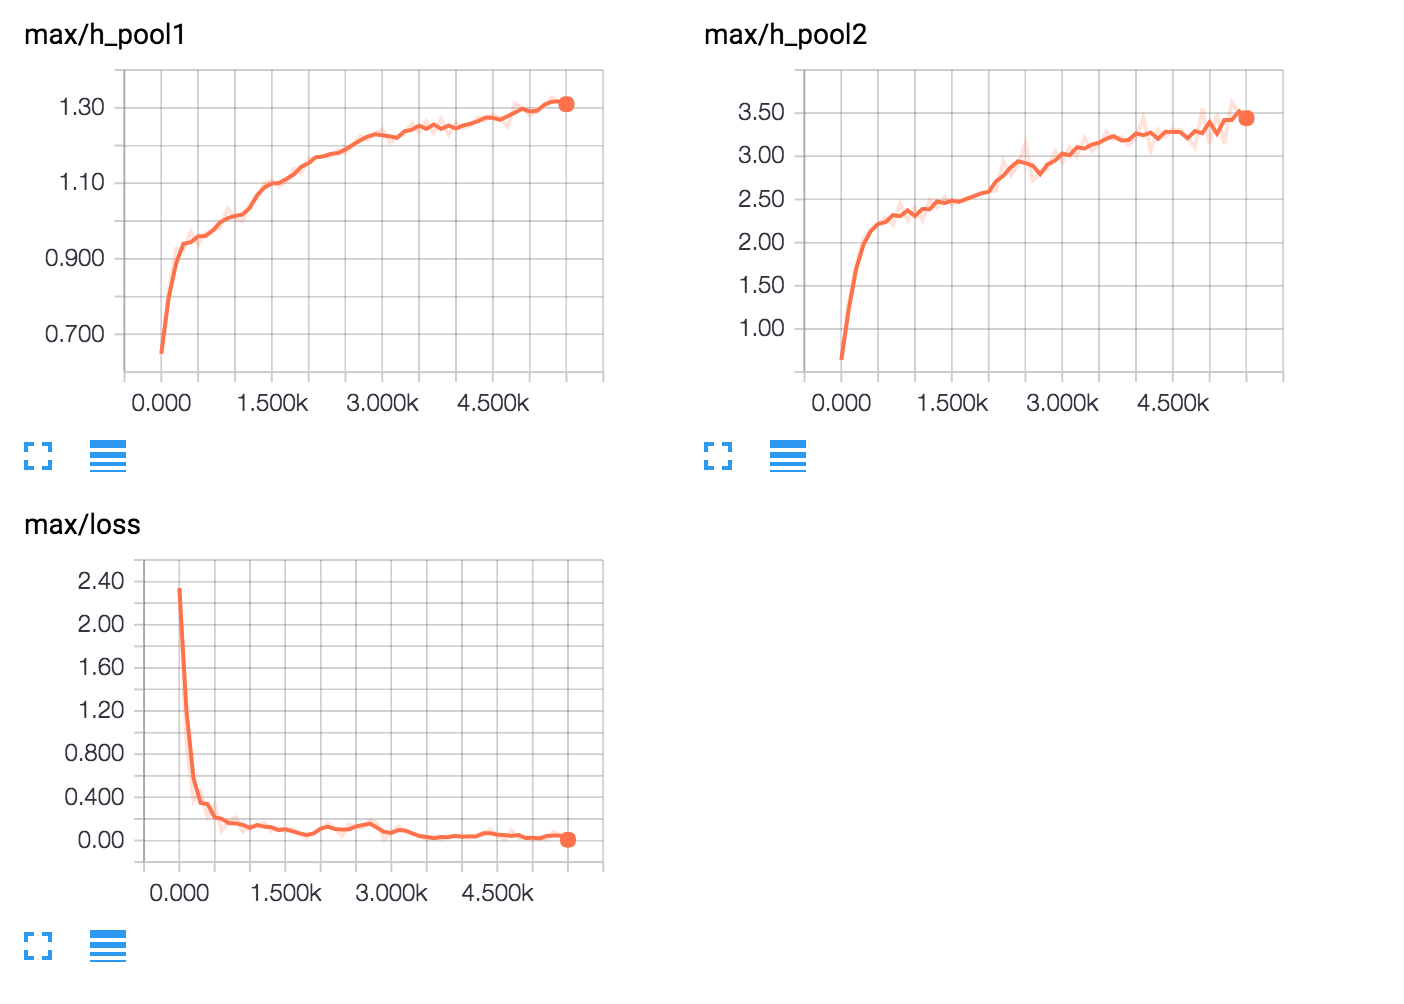
\includegraphics[scale=0.3]{bmax4.png}
\end{figure}
\begin{figure}[H]
  \caption{center}
  \centering
    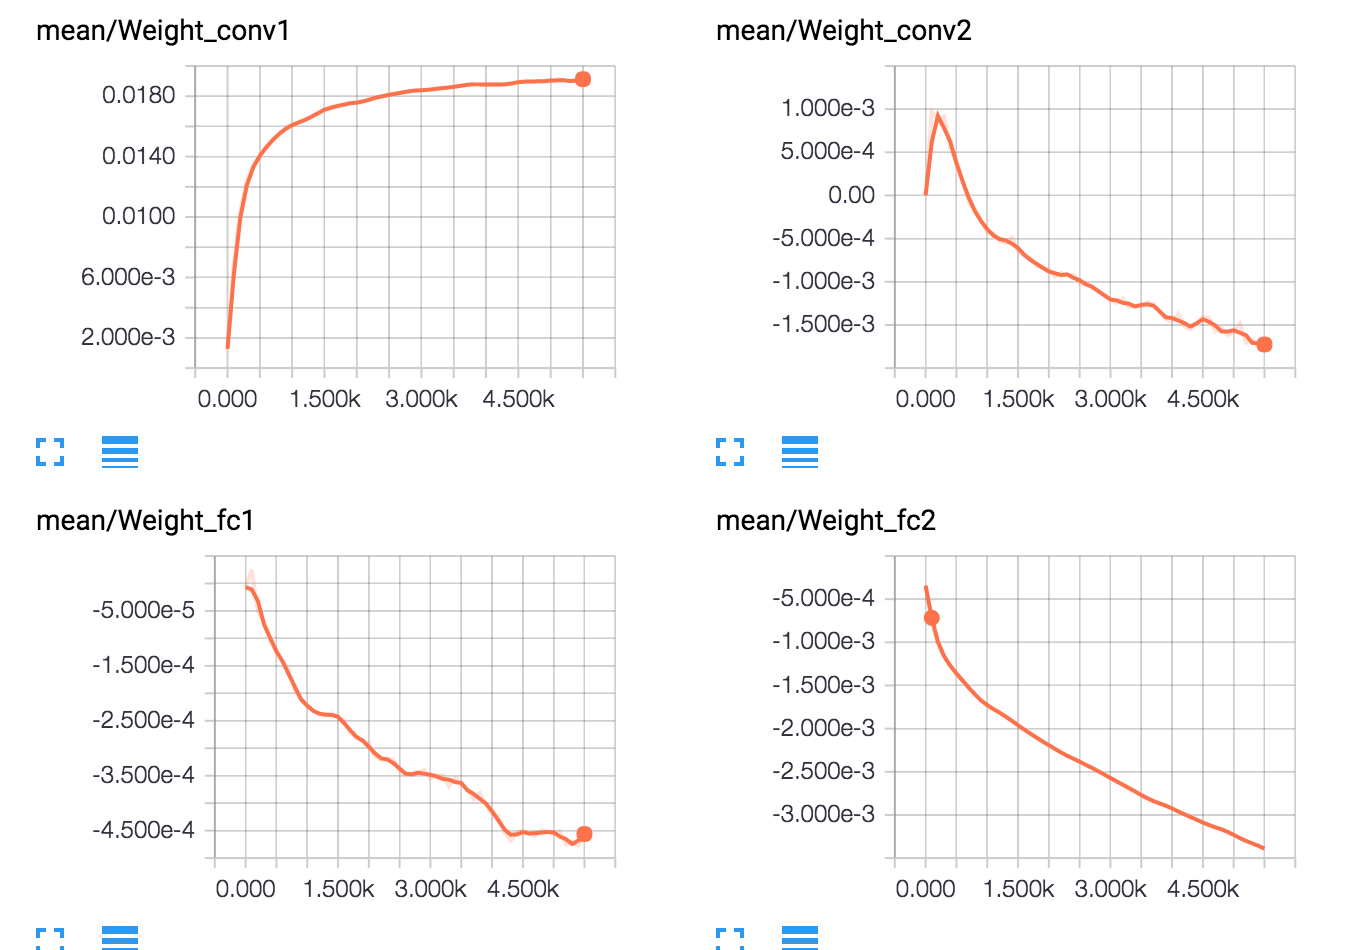
\includegraphics[scale=0.3]{bmean1.png}
\end{figure}
\begin{figure}[H]
  \caption{center}
  \centering
    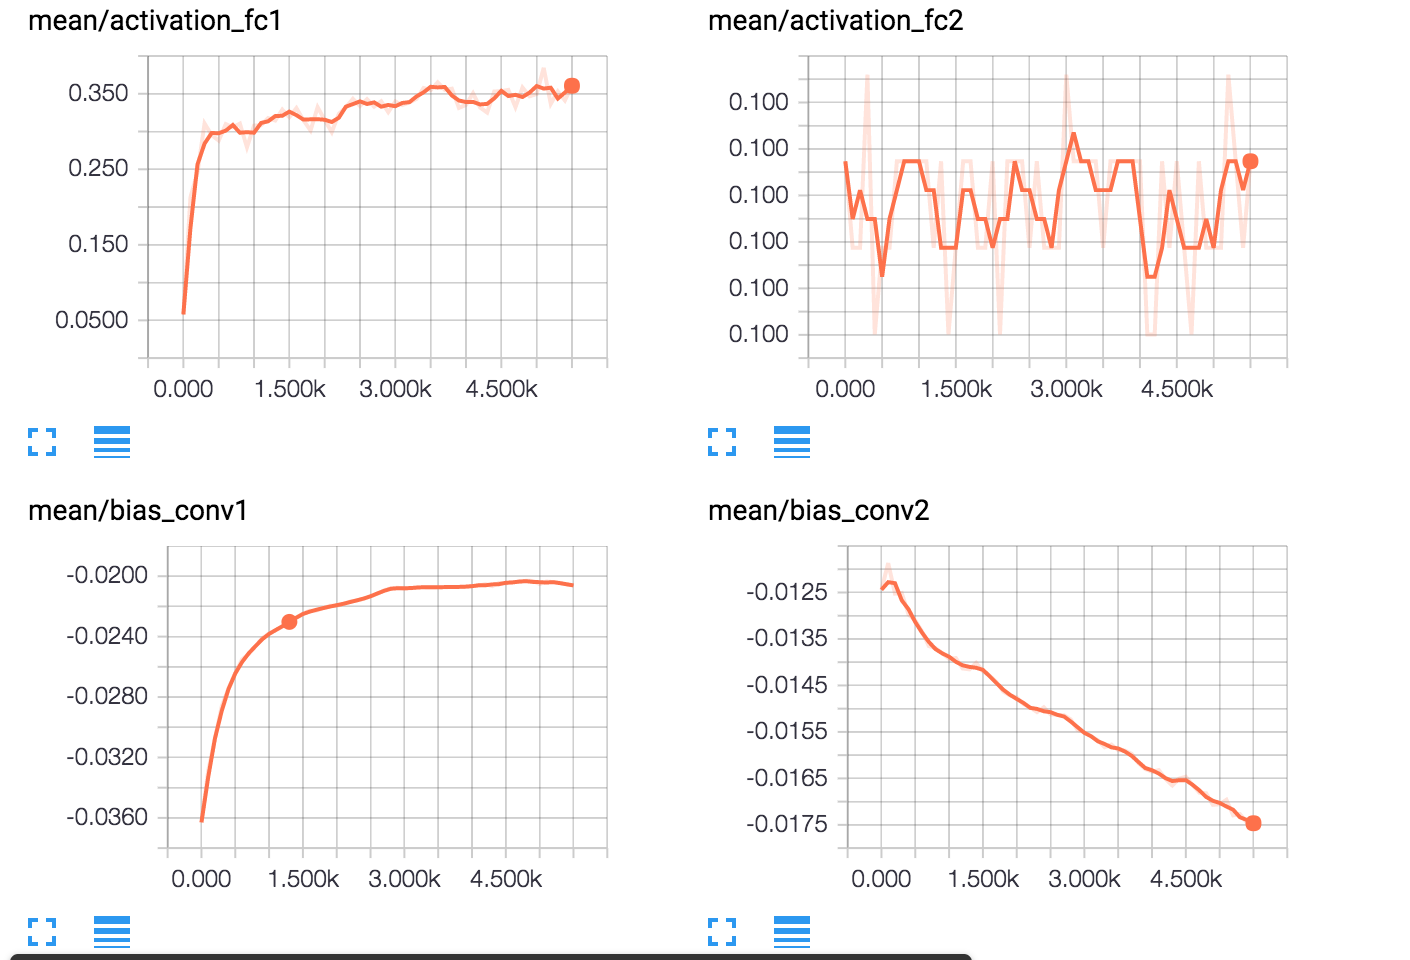
\includegraphics[scale=0.3]{beam2.png}
\end{figure}

\begin{figure}[H]
  \caption{center}
  \centering
    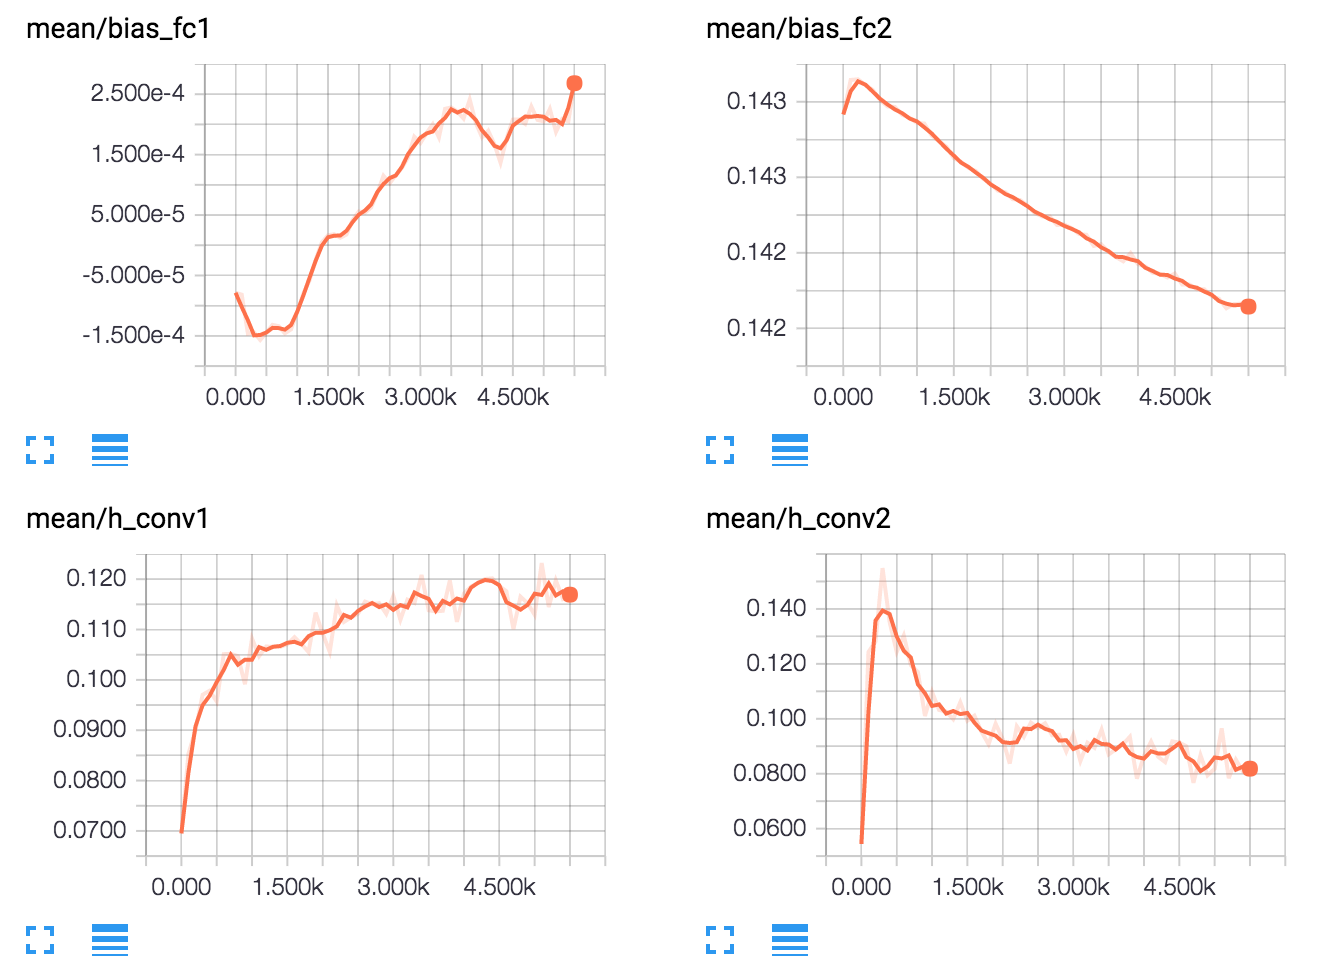
\includegraphics[scale=0.3]{beam3.png}
\end{figure}
\begin{figure}[H]
  \caption{center}
  \centering
    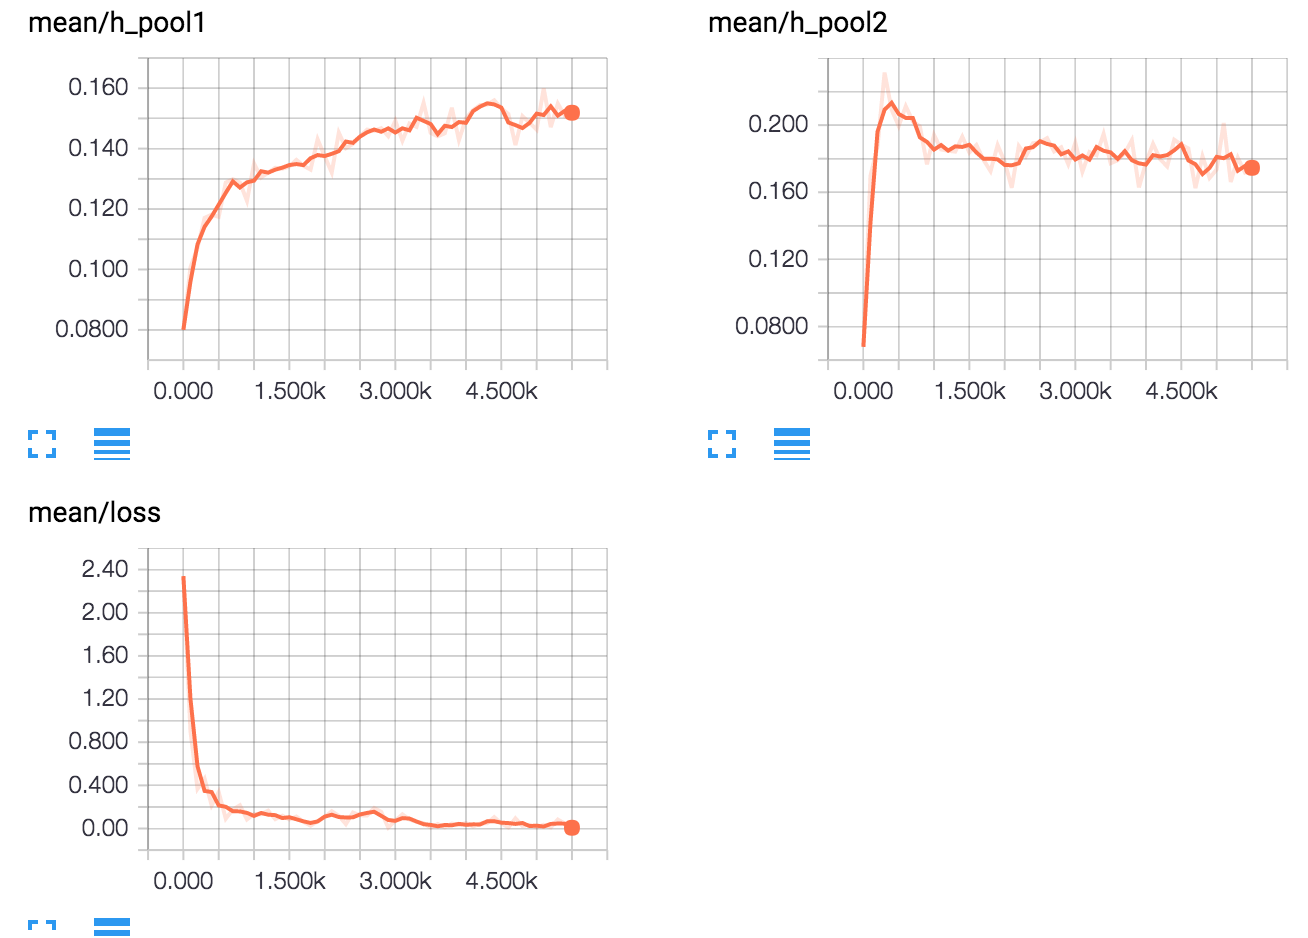
\includegraphics[scale=0.3]{bmean4.png}
\end{figure}
\begin{figure}[H]
  \caption{center}
  \centering
    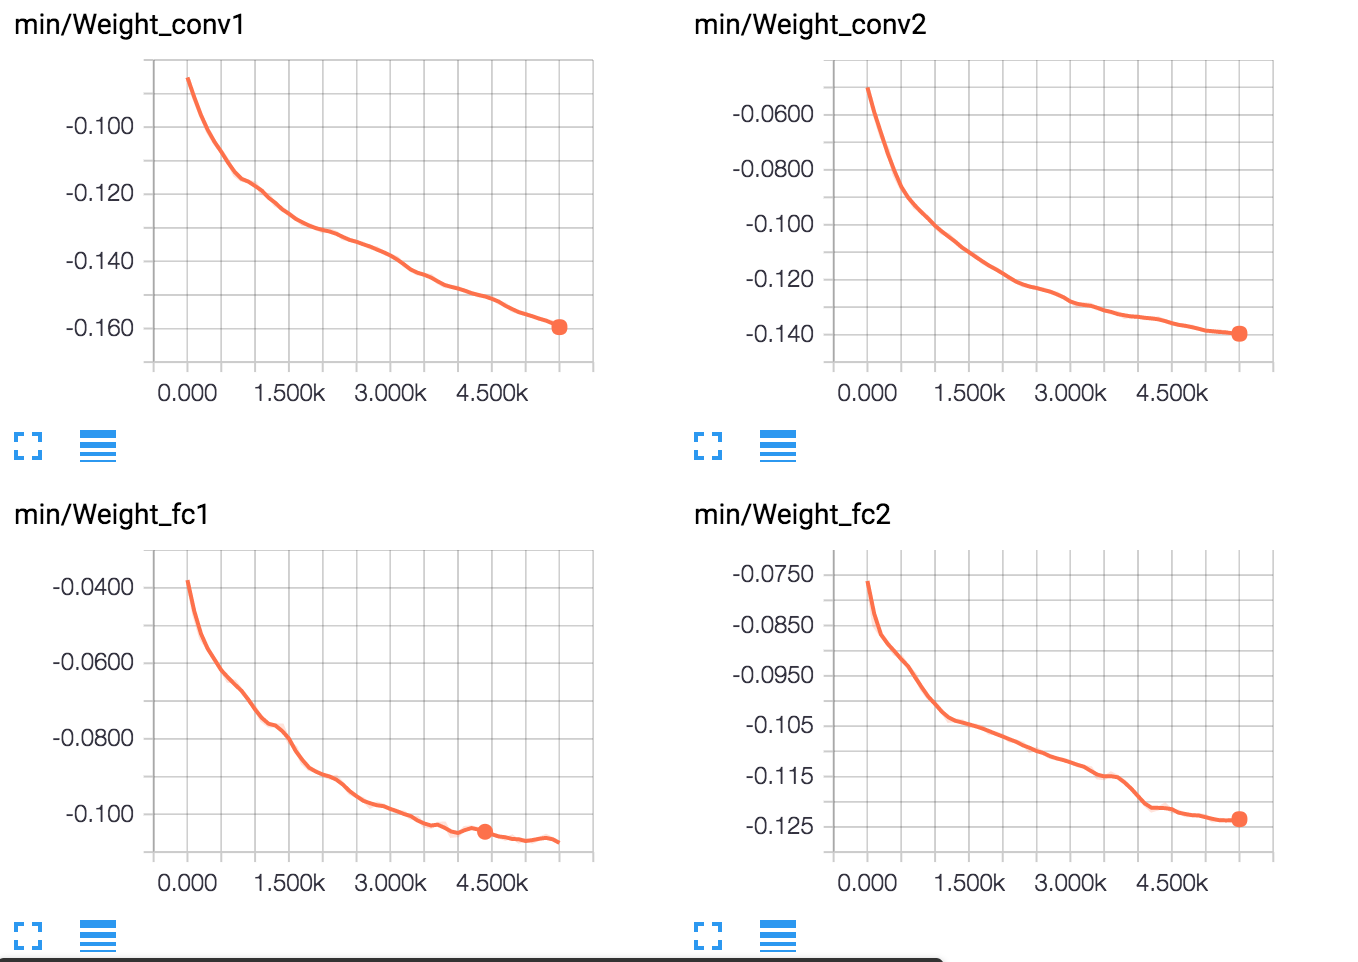
\includegraphics[scale=0.3]{bmin1.png}
\end{figure}
\begin{figure}[H]
  \caption{center}
  \centering
    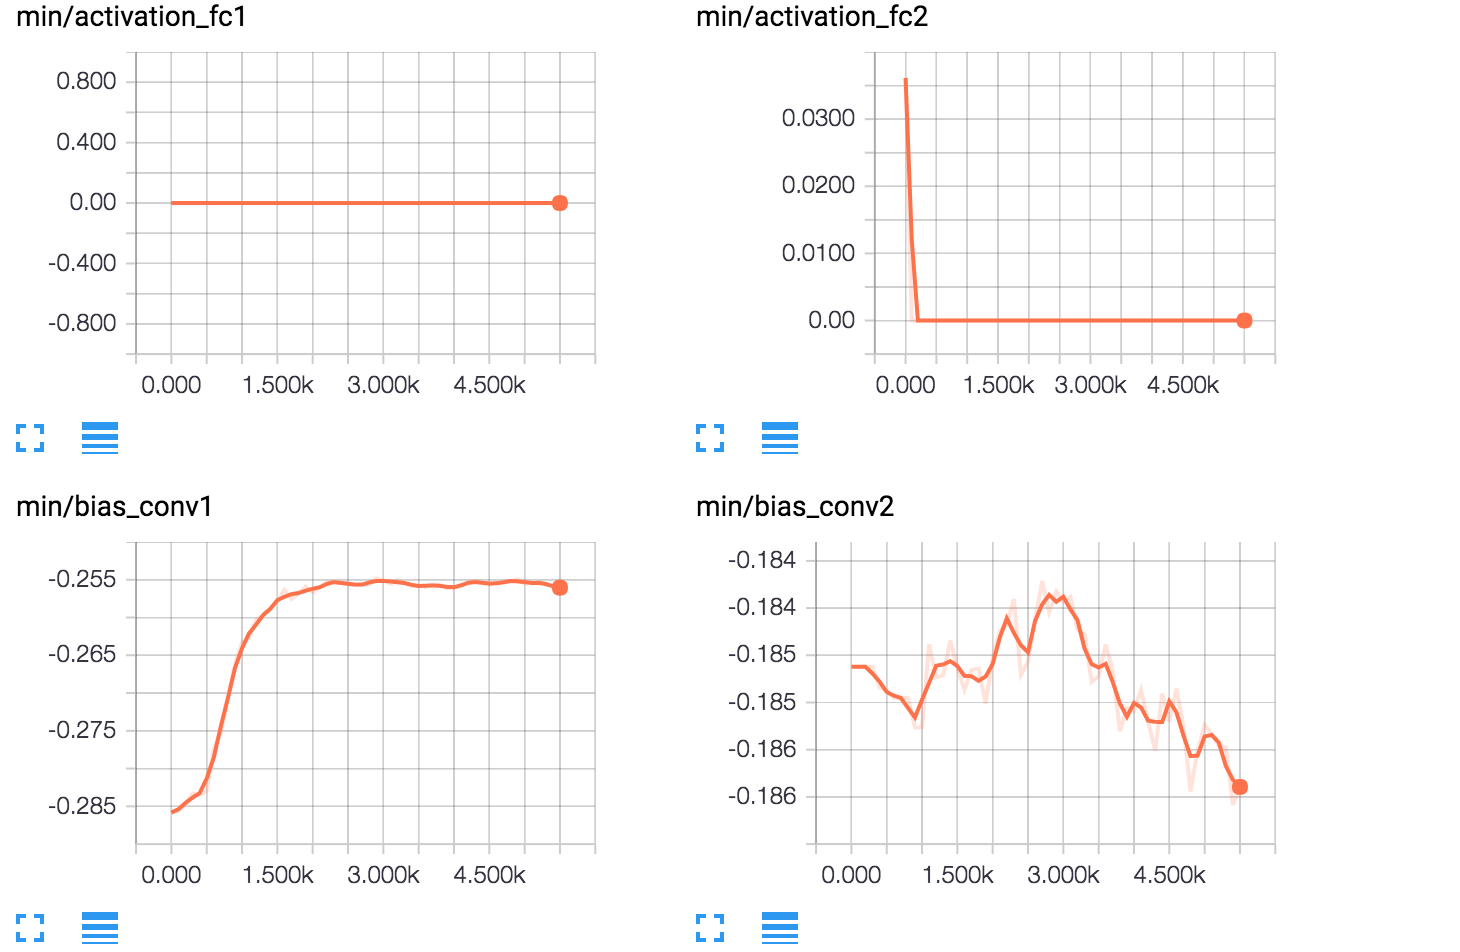
\includegraphics[scale=0.3]{bmin2.png}
\end{figure}
\begin{figure}[H]
  \caption{center}
  \centering
    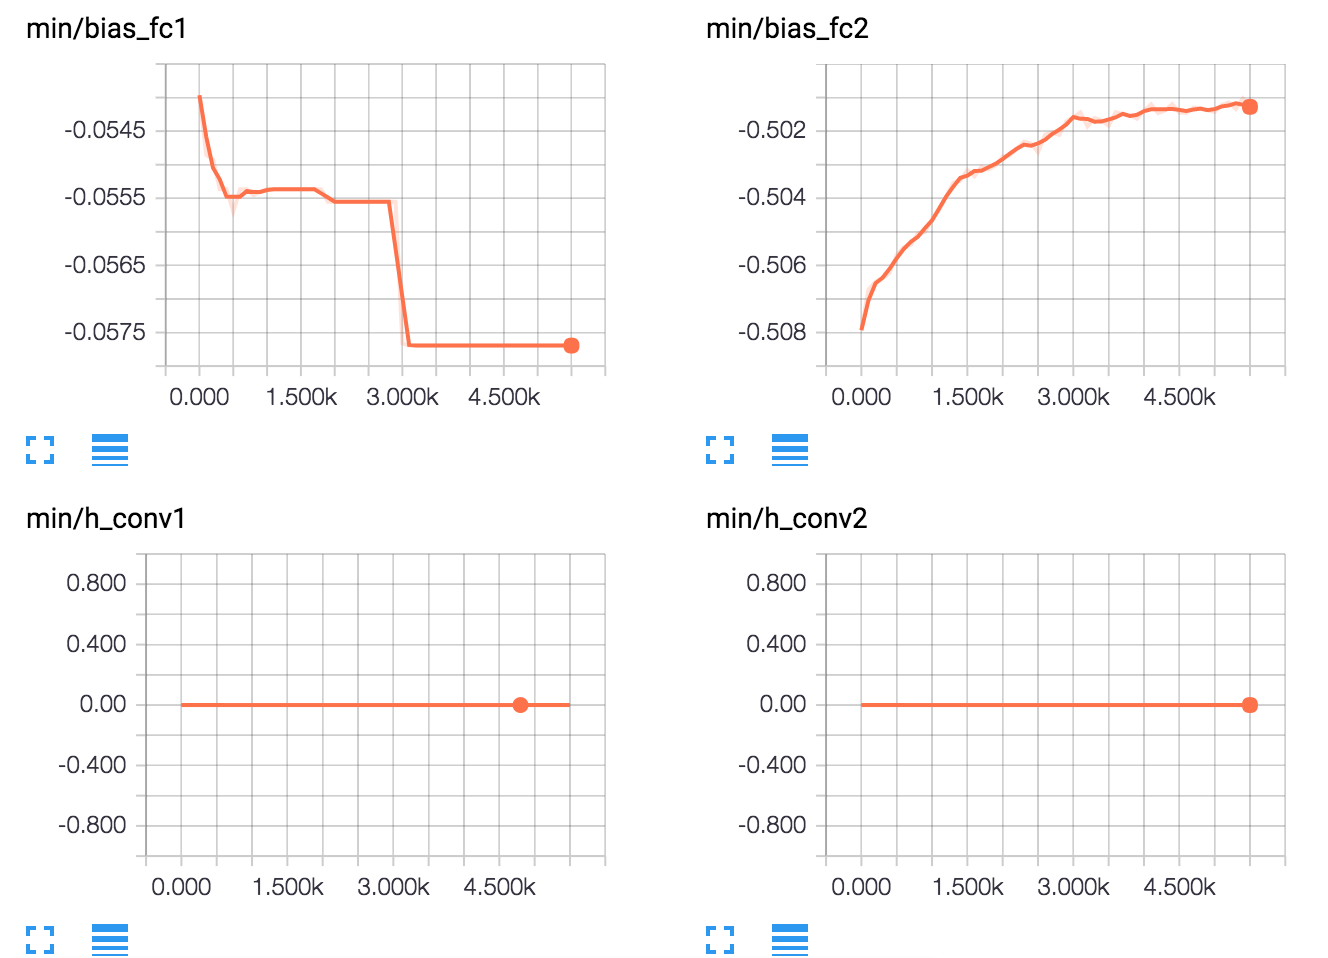
\includegraphics[scale=0.3]{bmin3.png}
\end{figure}
\begin{figure}[H]
  \caption{center}
  \centering
    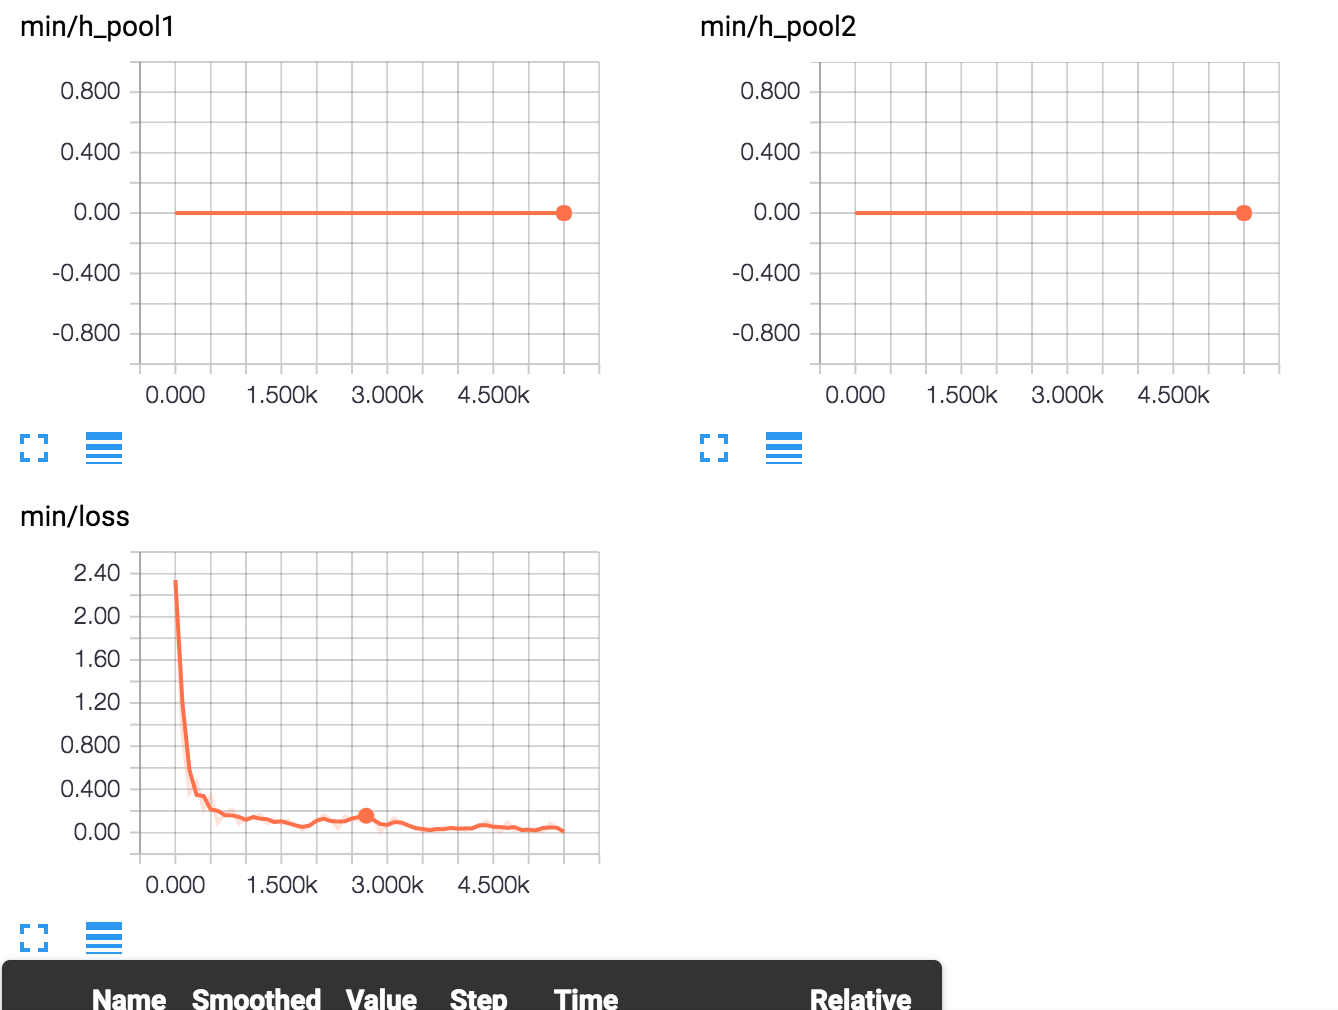
\includegraphics[scale=0.3]{bmin4.png}
\end{figure}
\begin{figure}[H]
  \caption{center}
  \centering
    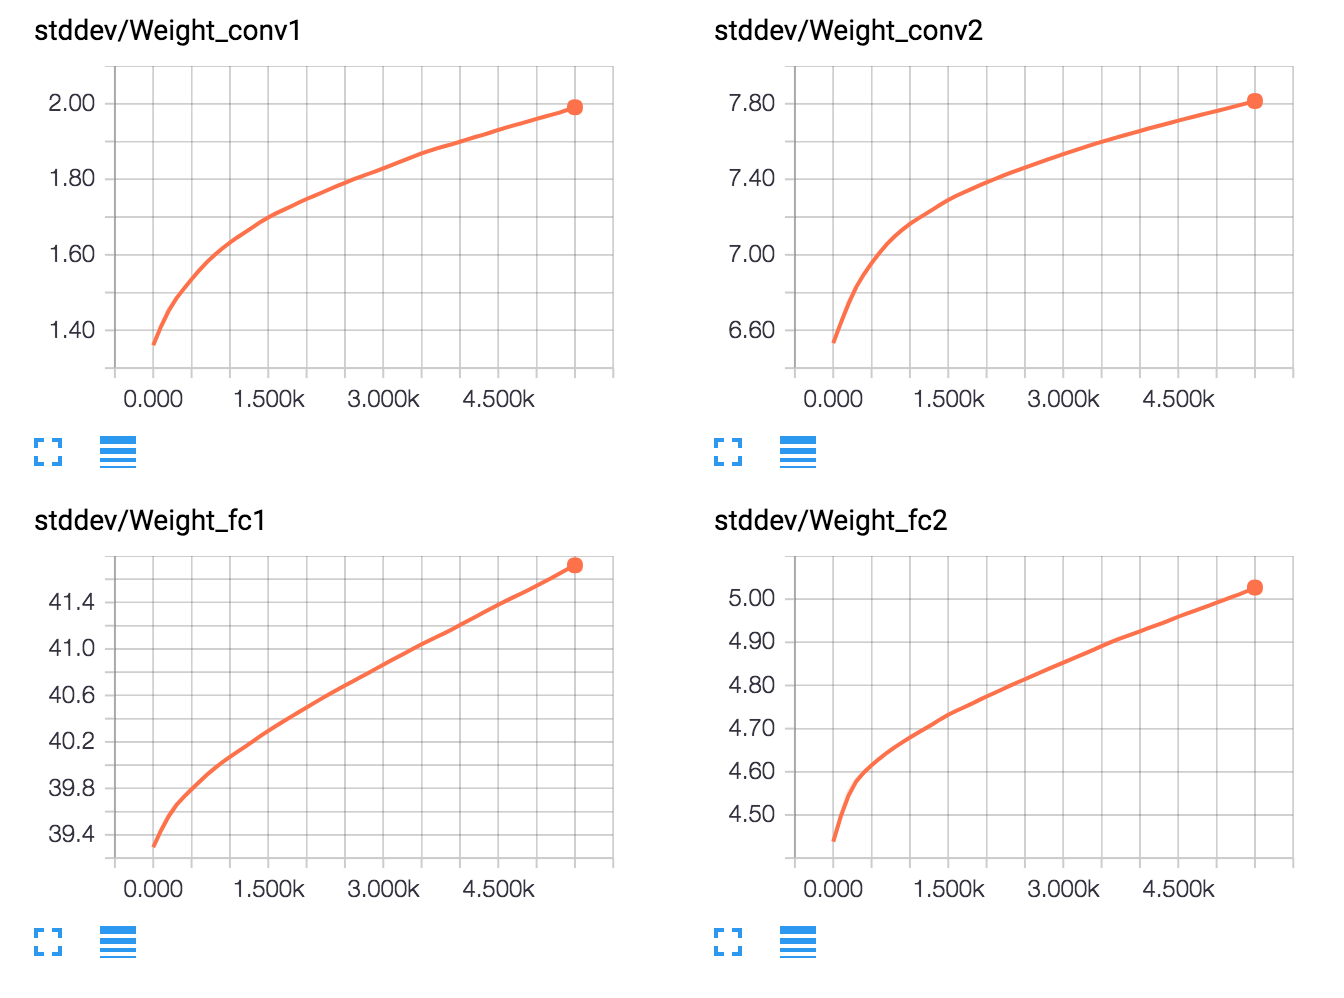
\includegraphics[scale=0.3]{bst1.png}
\end{figure}

\begin{figure}[H]
  \caption{center}
  \centering
    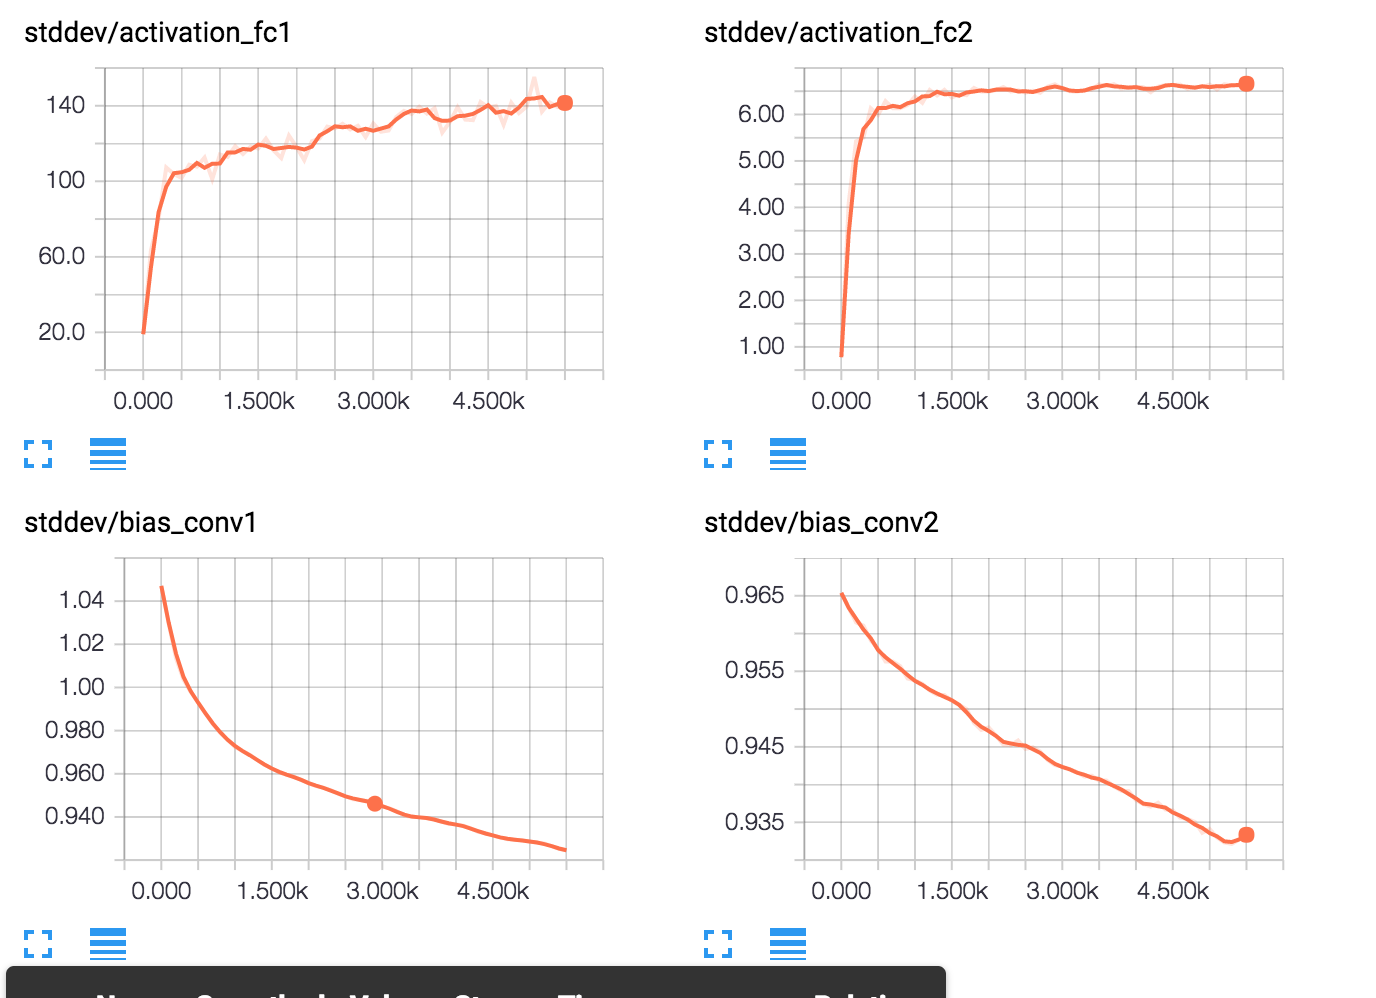
\includegraphics[scale=0.3]{bst2.png}
\end{figure}
\begin{figure}[H]
  \caption{center}
  \centering
    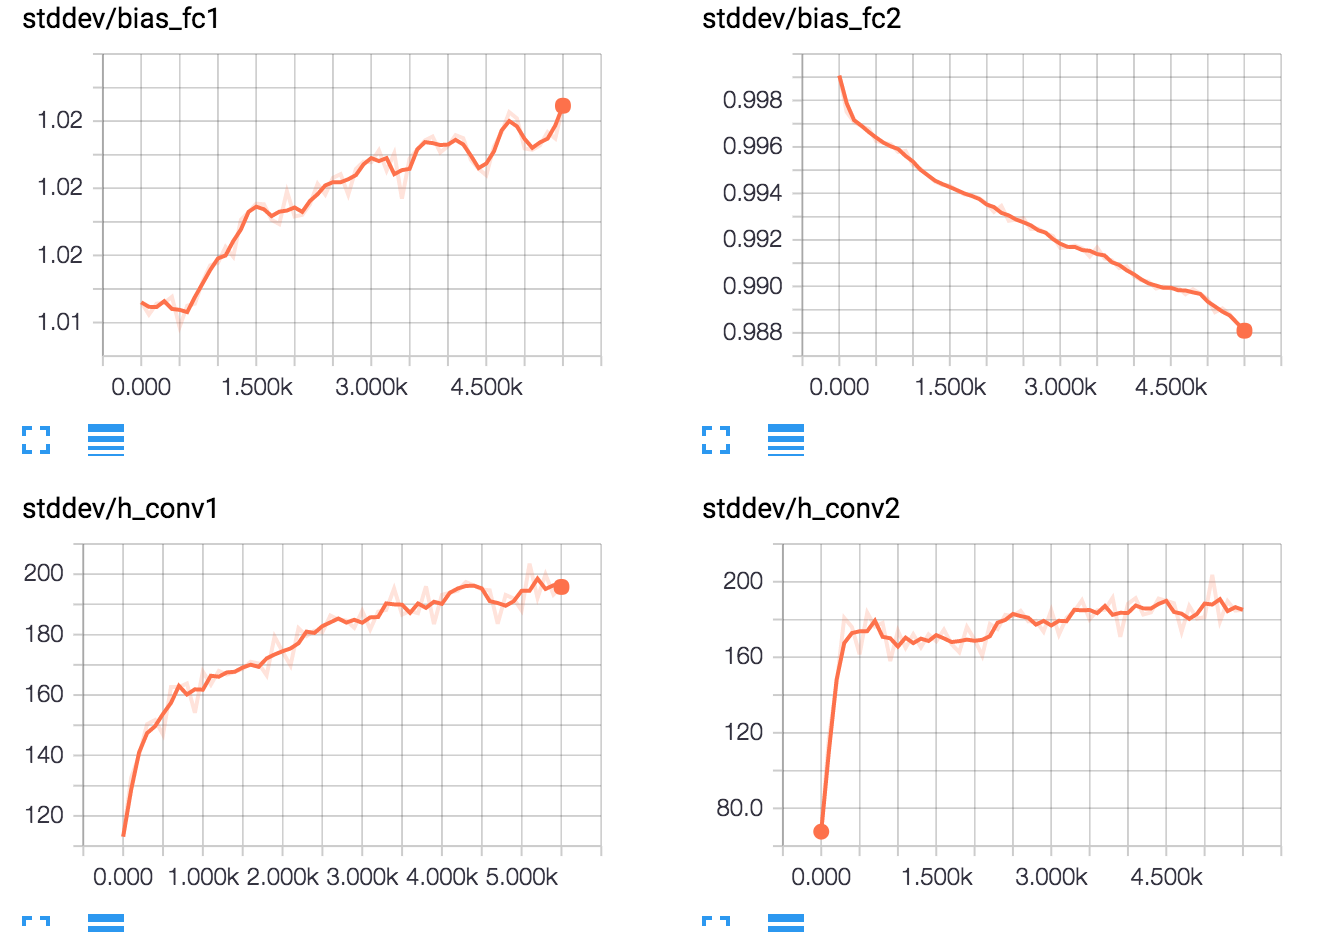
\includegraphics[scale=0.3]{bst3.png}
\end{figure}
\begin{figure}[H]
  \caption{center}
  \centering
    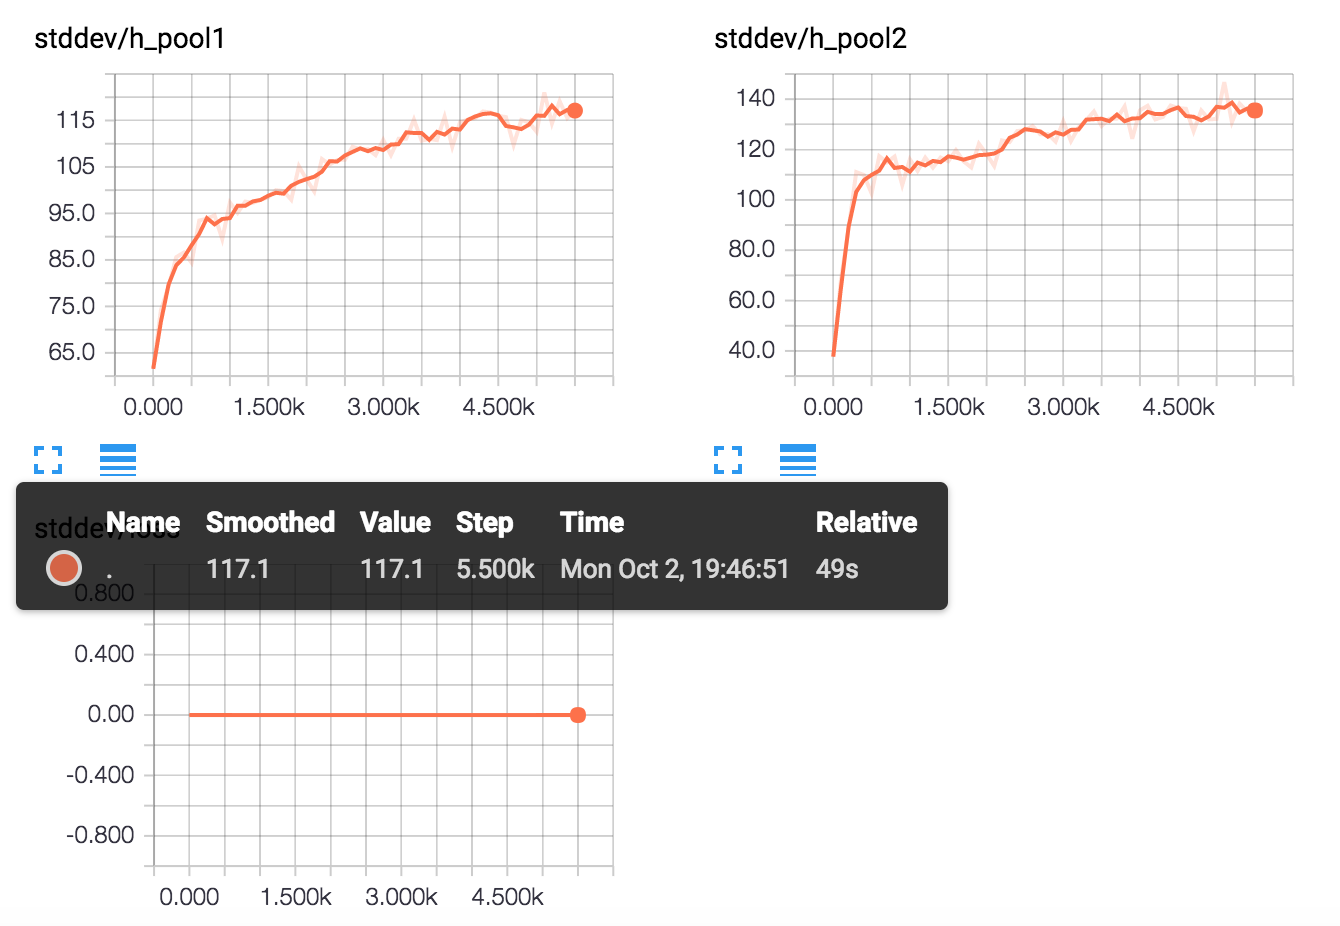
\includegraphics[scale=0.3]{bst4.png}
\end{figure}
I put the validation accuracy monitor in a son file called "valid"
And put parts of the plots here. 
\begin{figure}[H]
  \caption{center}
  \centering
    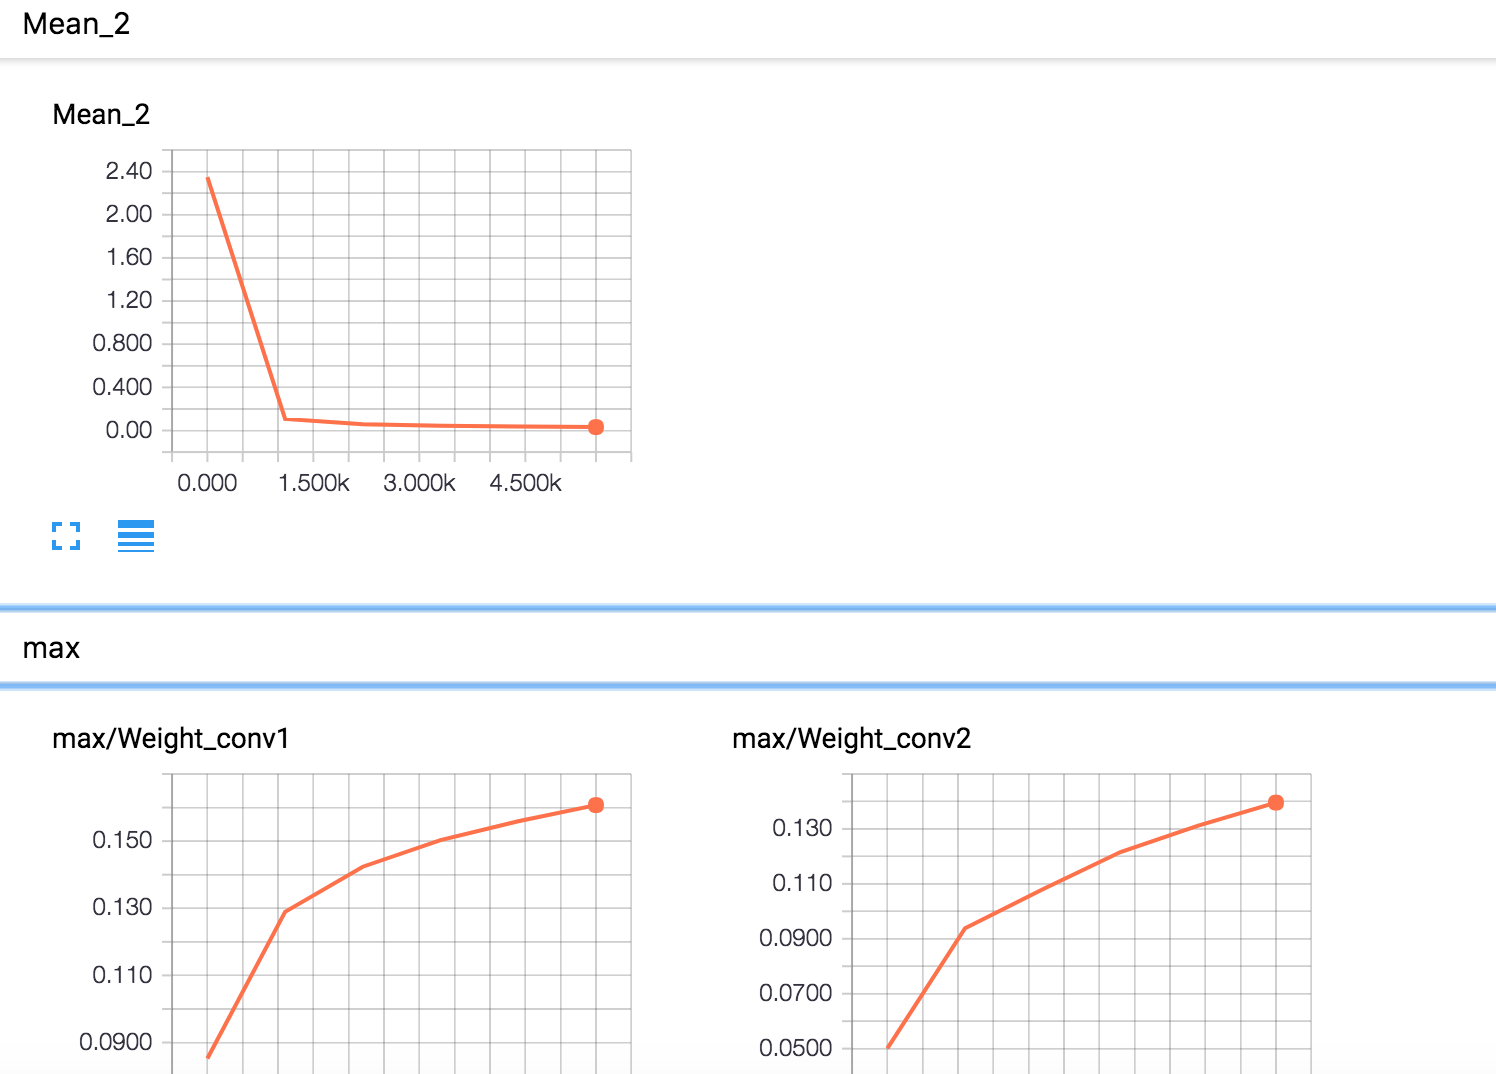
\includegraphics[scale=0.3]{validation.png}
\end{figure}



 \begin{lstlisting}  
step 3300, training accuracy 1
test accuracy 0.9853
validation accuracy 0.984
step 3400, training accuracy 0.96
step 3500, training accuracy 1
step 3600, training accuracy 1
step 3700, training accuracy 1
step 3800, training accuracy 0.98
step 3900, training accuracy 1
step 4000, training accuracy 1
step 4100, training accuracy 0.98
step 4200, training accuracy 0.98
step 4300, training accuracy 1
step 4400, training accuracy 1
test accuracy 0.988
validation accuracy 0.9878
step 4500, training accuracy 1
step 4600, training accuracy 1
step 4700, training accuracy 0.98
step 4800, training accuracy 0.98
step 4900, training accuracy 1
step 5000, training accuracy 1
step 5100, training accuracy 0.98
step 5200, training accuracy 1
step 5300, training accuracy 1
step 5400, training accuracy 0.98
step 5500, training accuracy 1
test accuracy 0.9899
validation accuracy 0.989
test accuracy 0.9899
The training takes 54.957134 second to finish
 \end{lstlisting}  



\subsection{C}
I use sigmoid function, RMSPropOptimizer. After 5500 training
step 5400, training accuracy 0.98
step 5500, training accuracy 0.98
test accuracy 0.9454
validation accuracy 0.95
The training takes 106.673226 second to finish. The accuracy goes up slowly at the begining. 


FIGURES:
\begin{figure}[H]
  \caption{center}
  \centering
    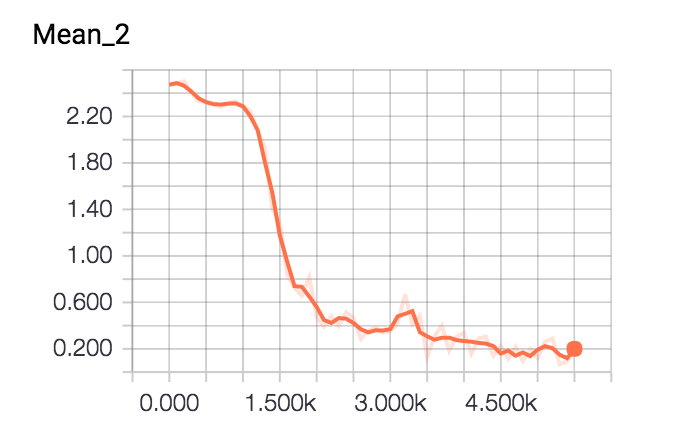
\includegraphics[scale=0.3]{mean2.png}
\end{figure}
\begin{figure}[H]
  \caption{center}
  \centering
    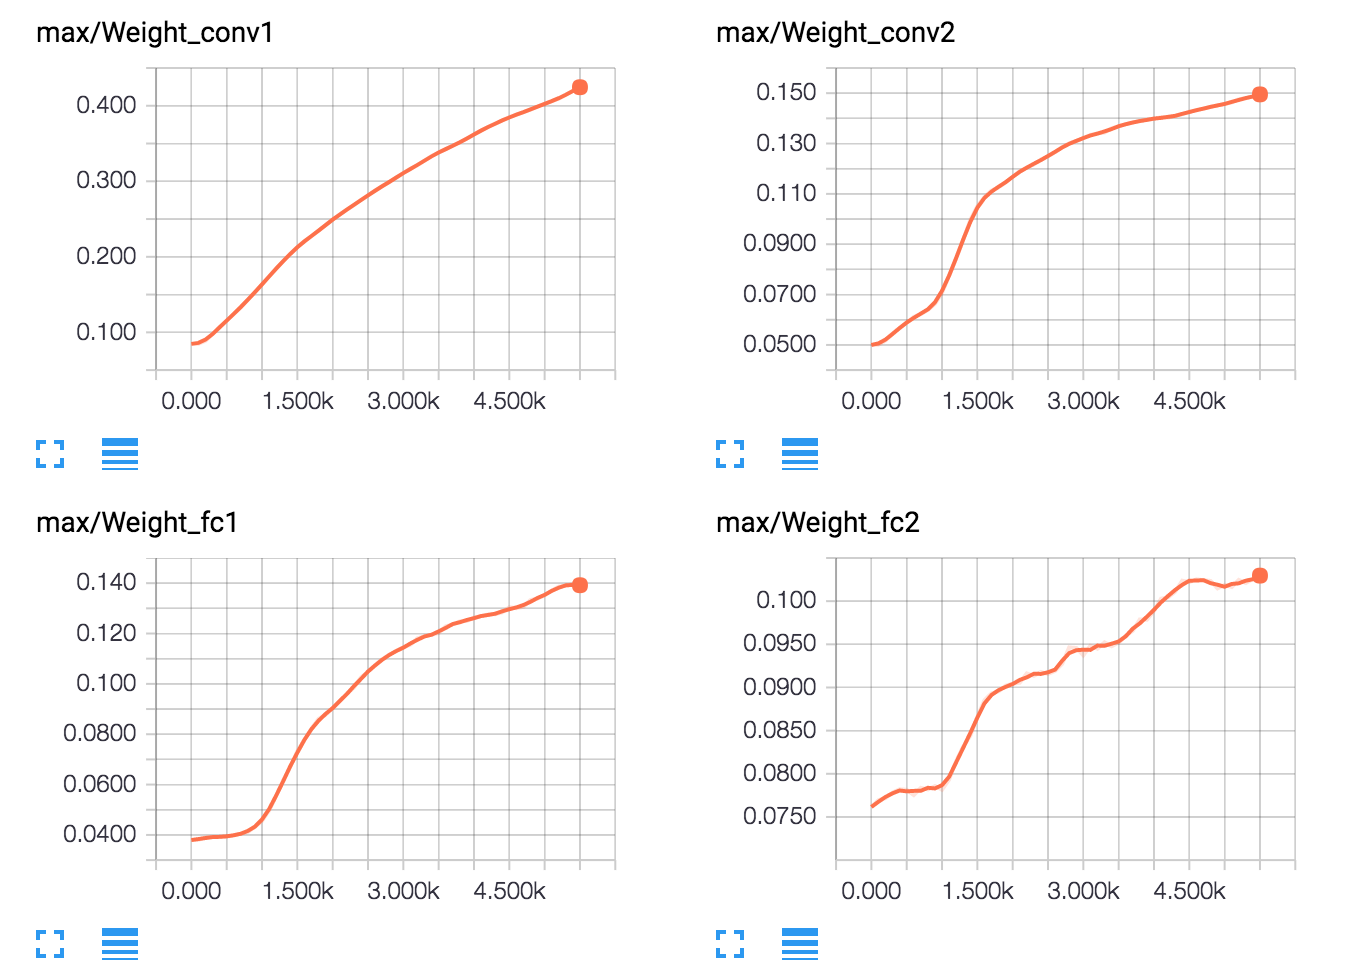
\includegraphics[scale=0.3]{weight.png}
\end{figure}
\begin{figure}[H]
  \caption{center}
  \centering
    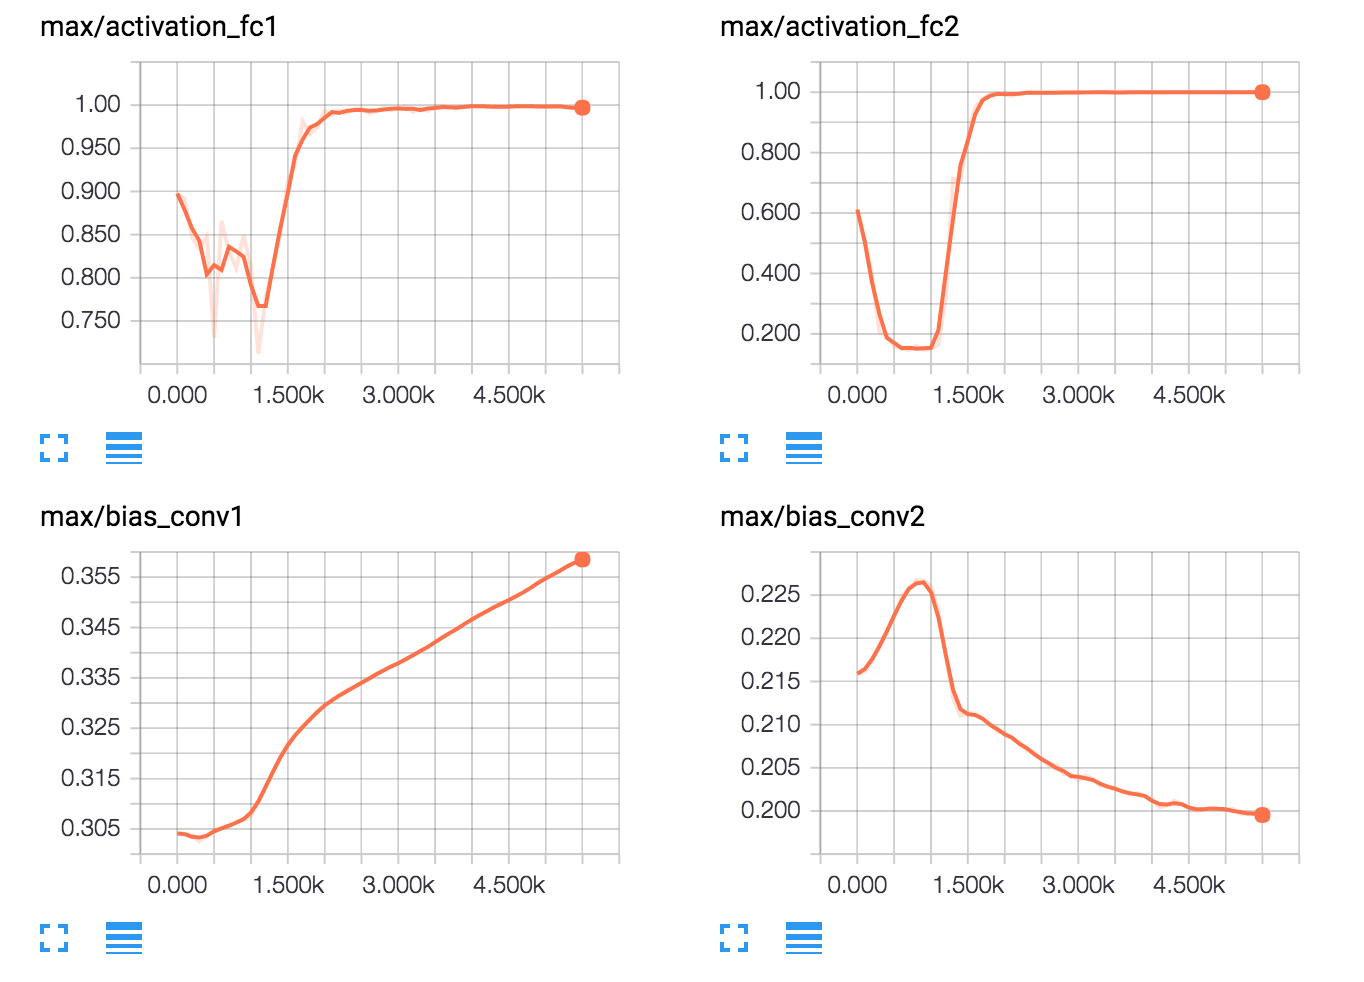
\includegraphics[scale=0.3]{w2.png}
\end{figure}
\begin{figure}[H]
  \caption{center}
  \centering
    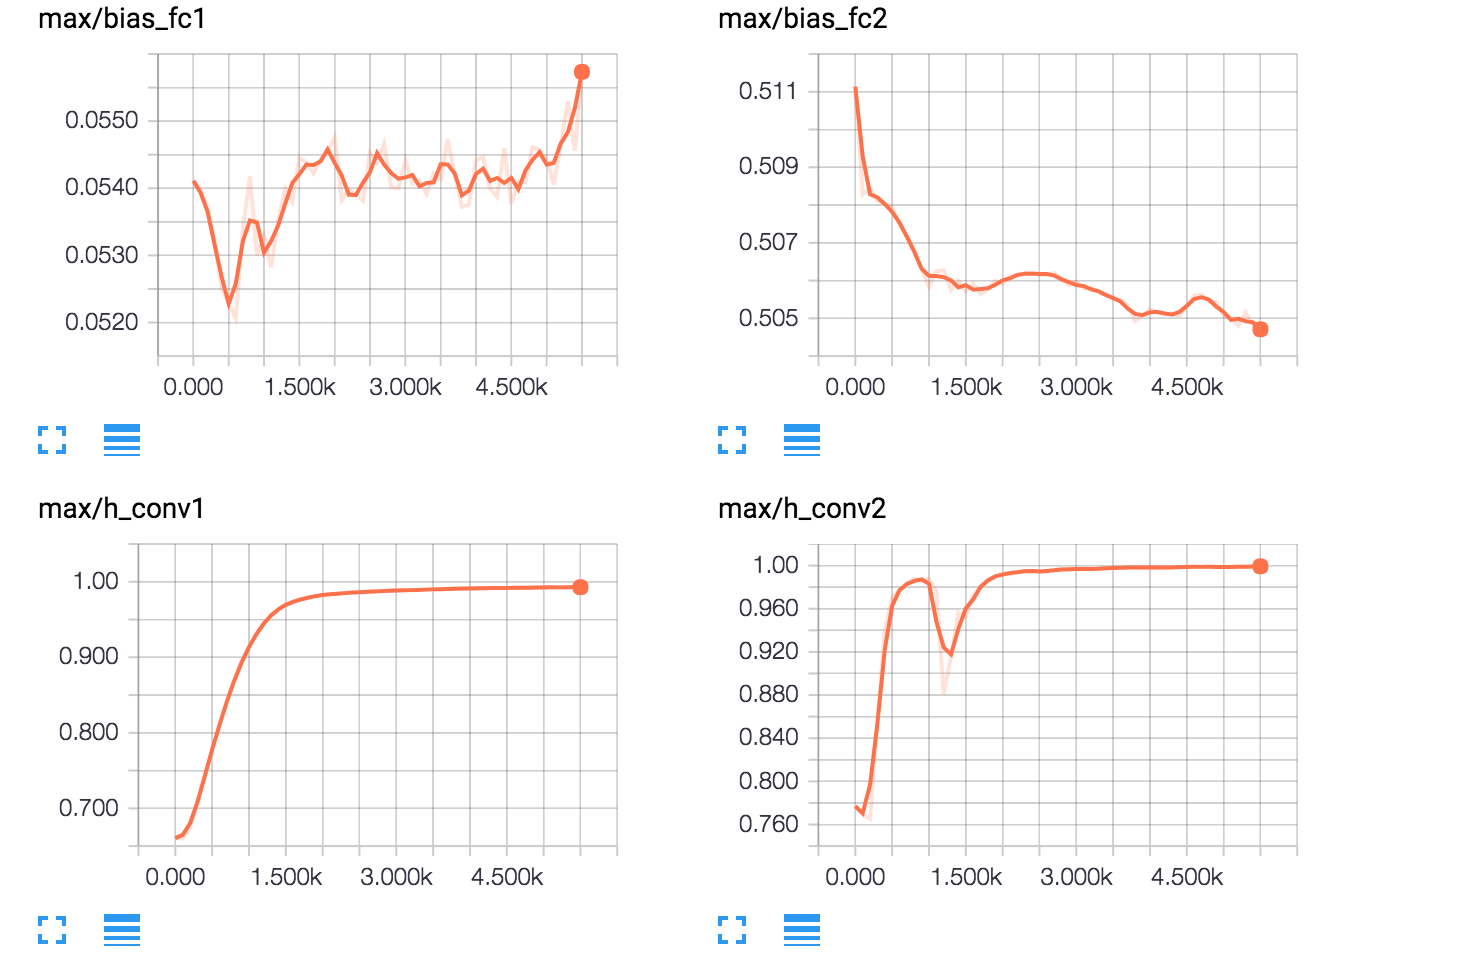
\includegraphics[scale=0.3]{b1.png}
\end{figure}
\begin{figure}[H]
  \caption{center}
  \centering
    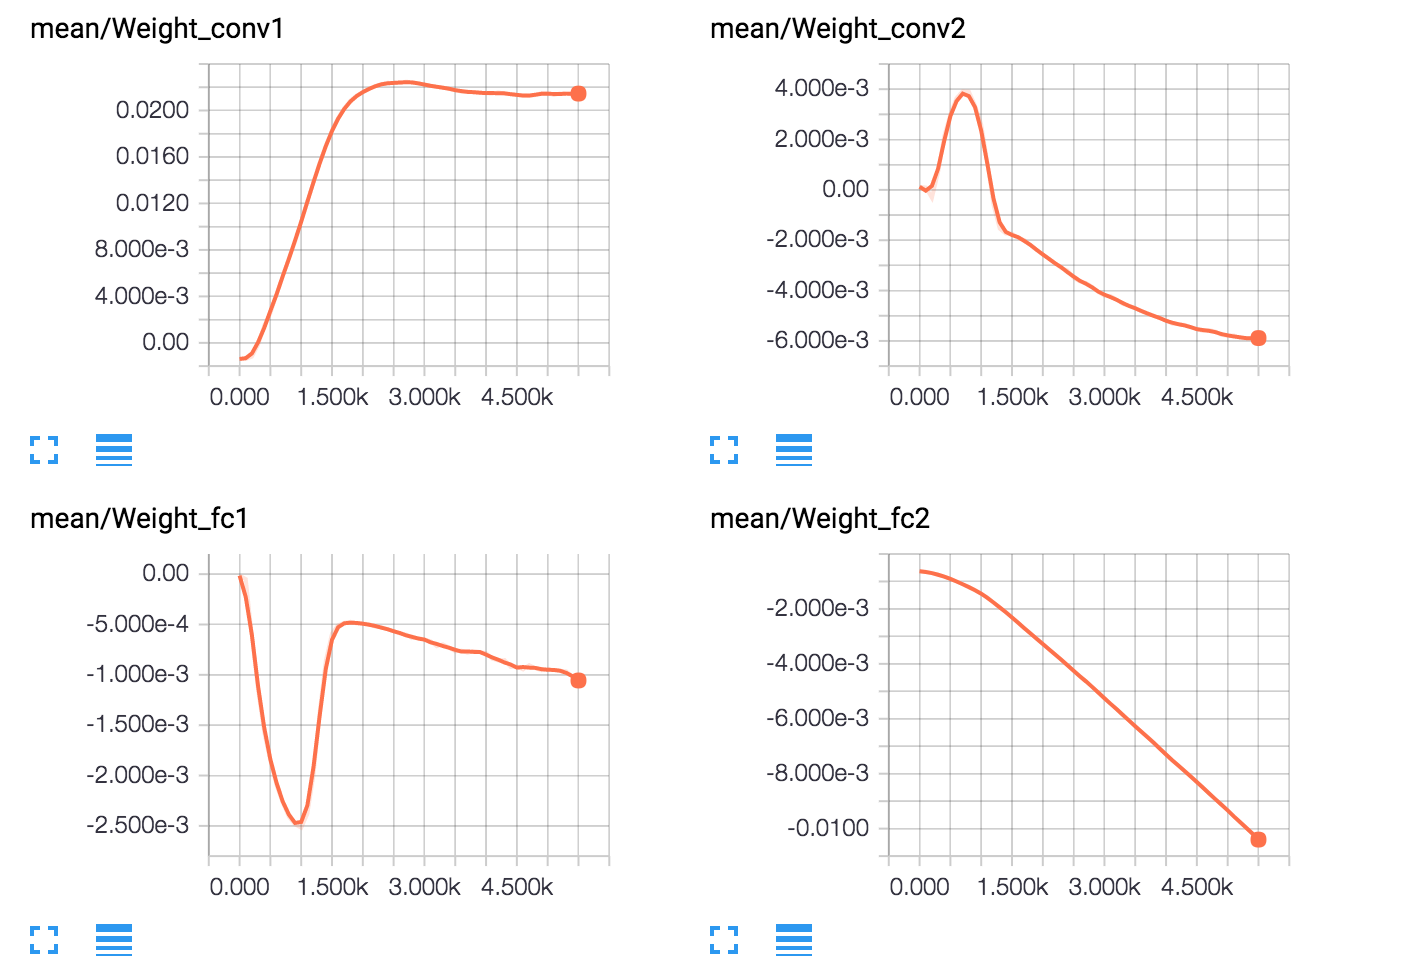
\includegraphics[scale=0.3]{mean.png}
\end{figure}
\begin{figure}[H]
  \caption{center}
  \centering
    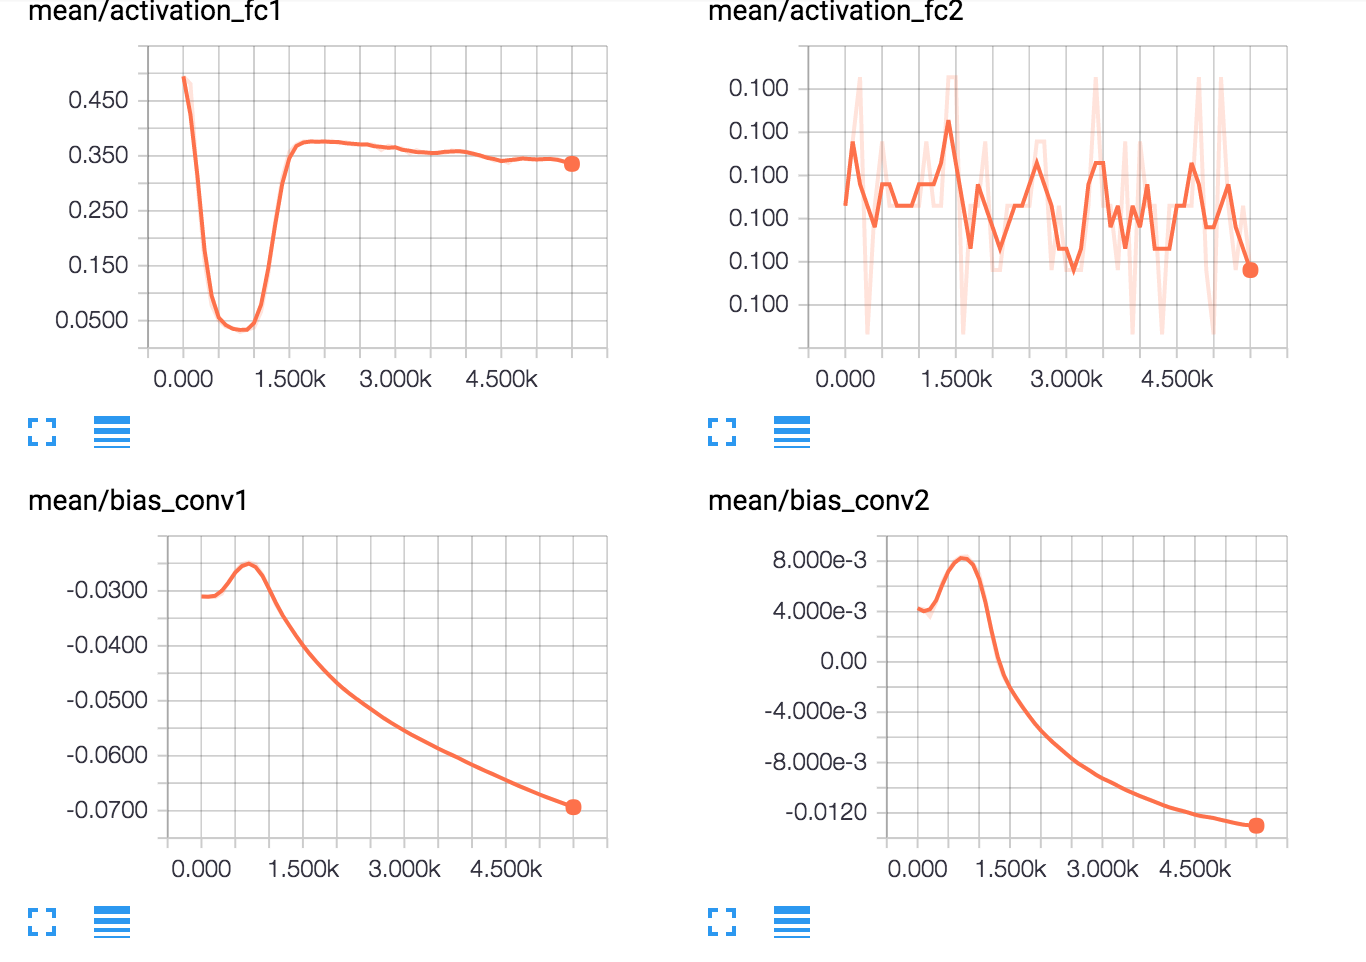
\includegraphics[scale=0.3]{mean3.png}
\end{figure}
\begin{figure}[H]
  \caption{center}
  \centering
    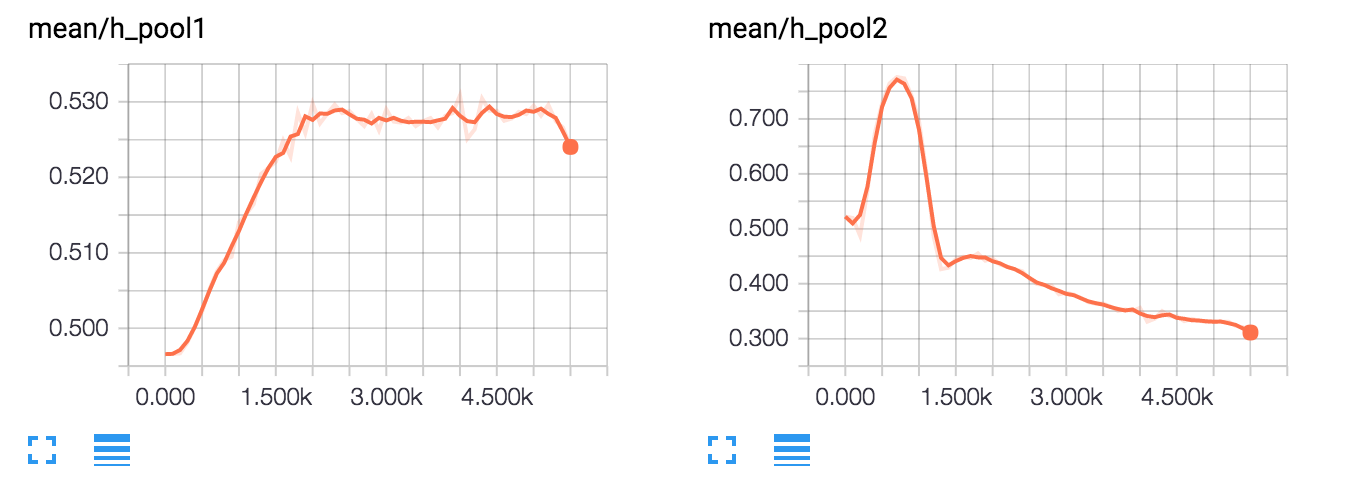
\includegraphics[scale=0.3]{mean4.png}
\end{figure}
\begin{figure}[H]
  \caption{center}
  \centering
    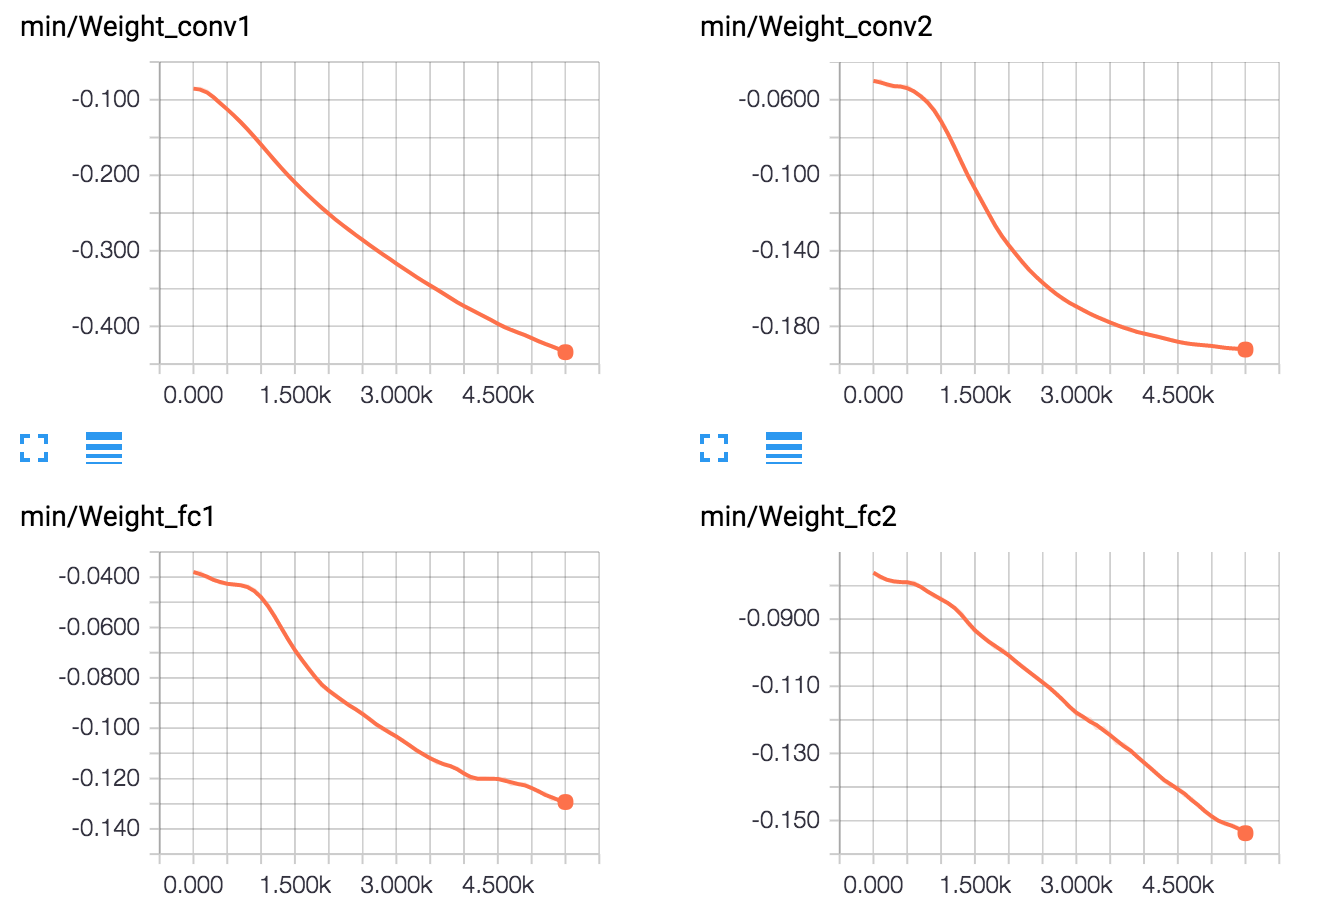
\includegraphics[scale=0.3]{min.png}
\end{figure}
\begin{figure}[H]
  \caption{center}
  \centering
    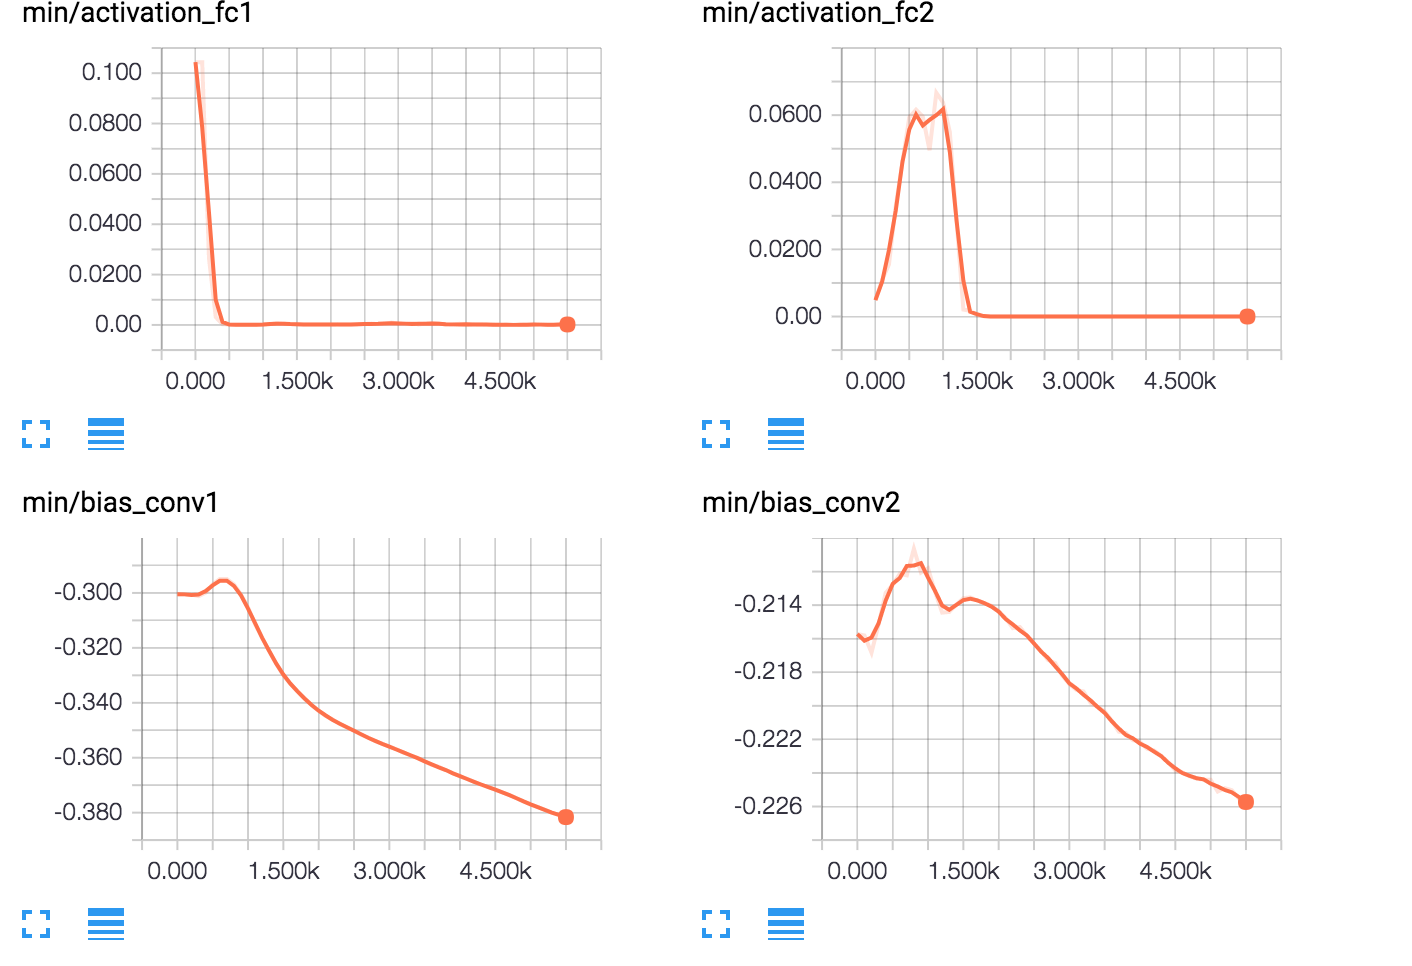
\includegraphics[scale=0.3]{min2.png}
\end{figure}
\begin{figure}[H]
  \caption{center}
  \centering
    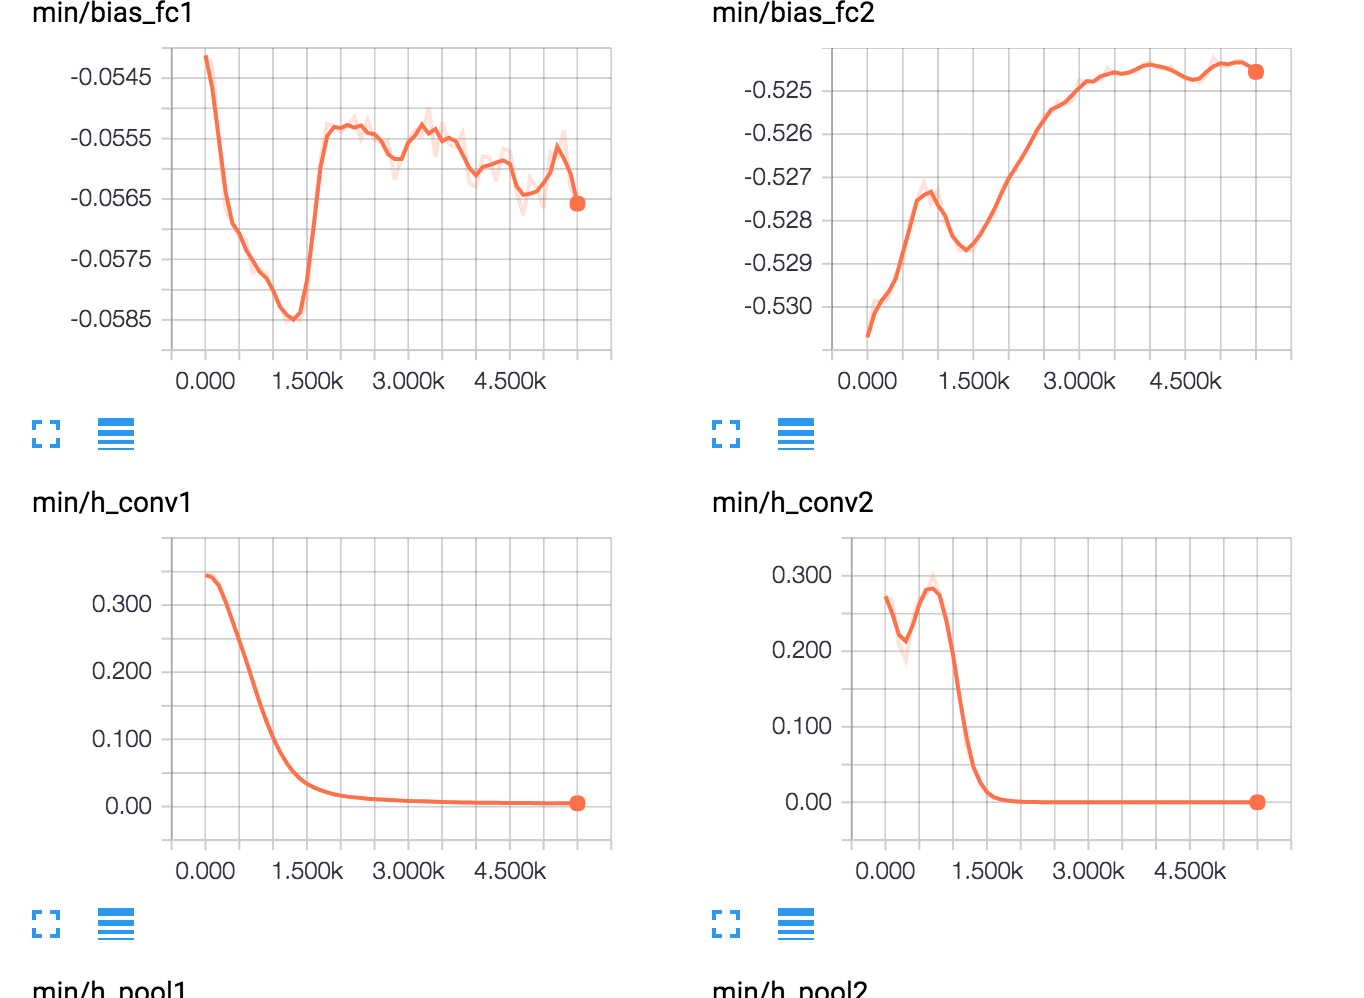
\includegraphics[scale=0.3]{min3.png}
\end{figure}
\begin{figure}[H]
  \caption{center}
  \centering
    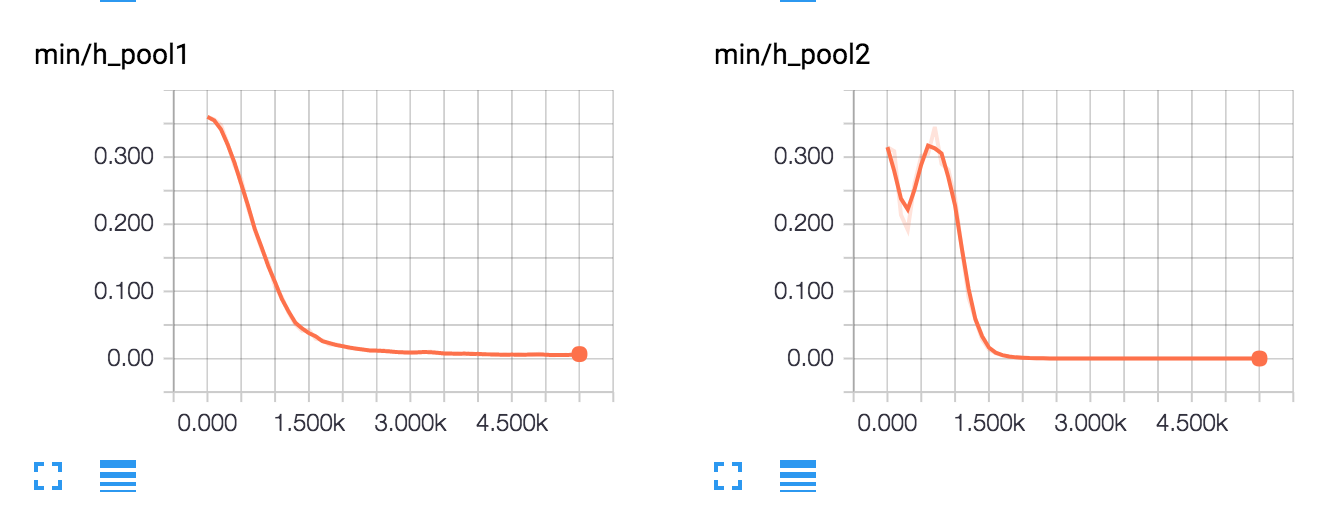
\includegraphics[scale=0.3]{min4.png}
\end{figure}
\begin{figure}[H]
  \caption{center}
  \centering
    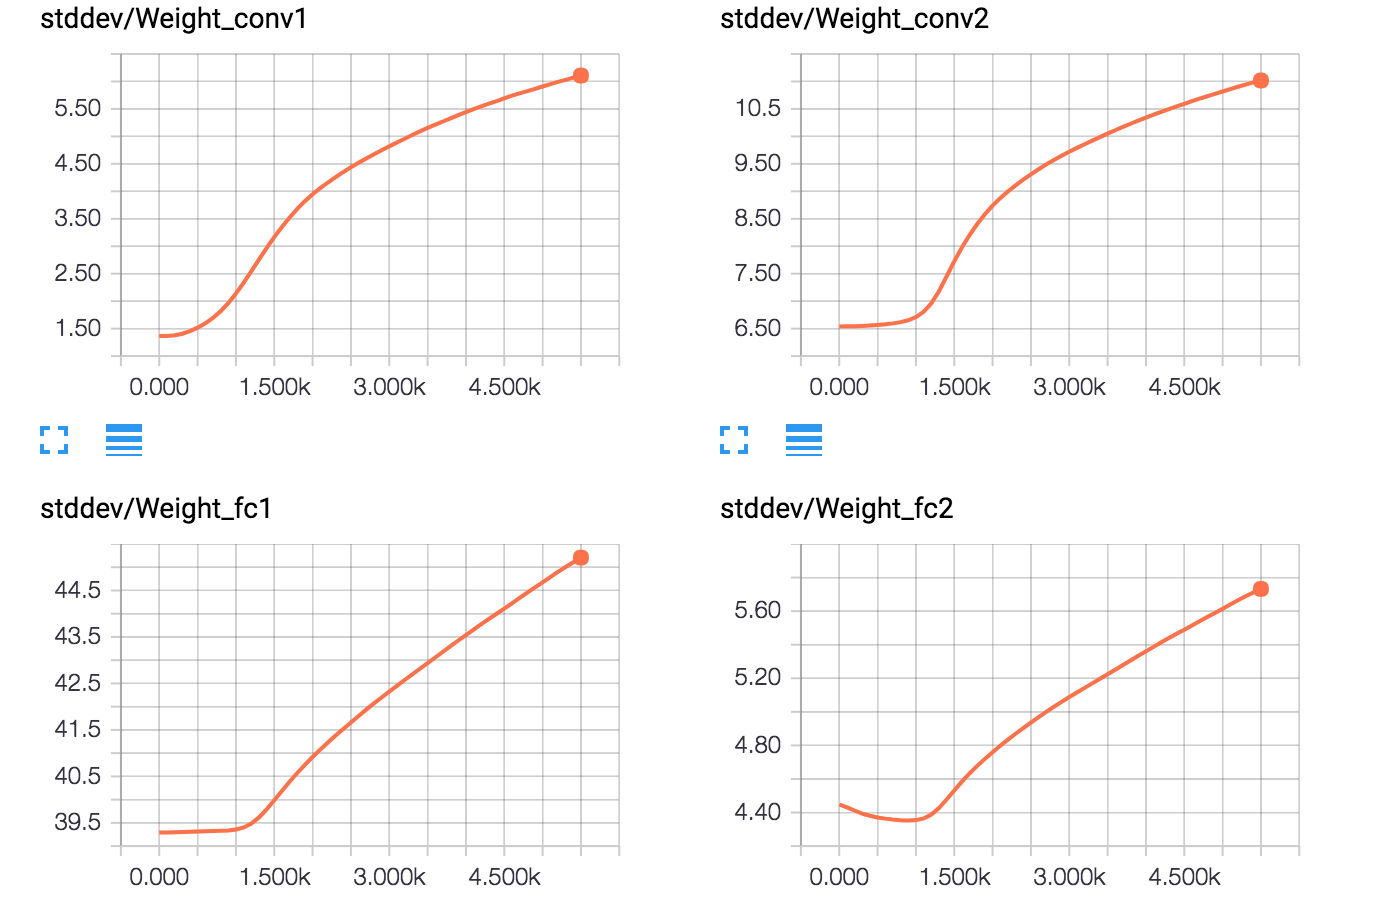
\includegraphics[scale=0.3]{st1.png}
\end{figure}
\begin{figure}[H]
  \caption{center}
  \centering
    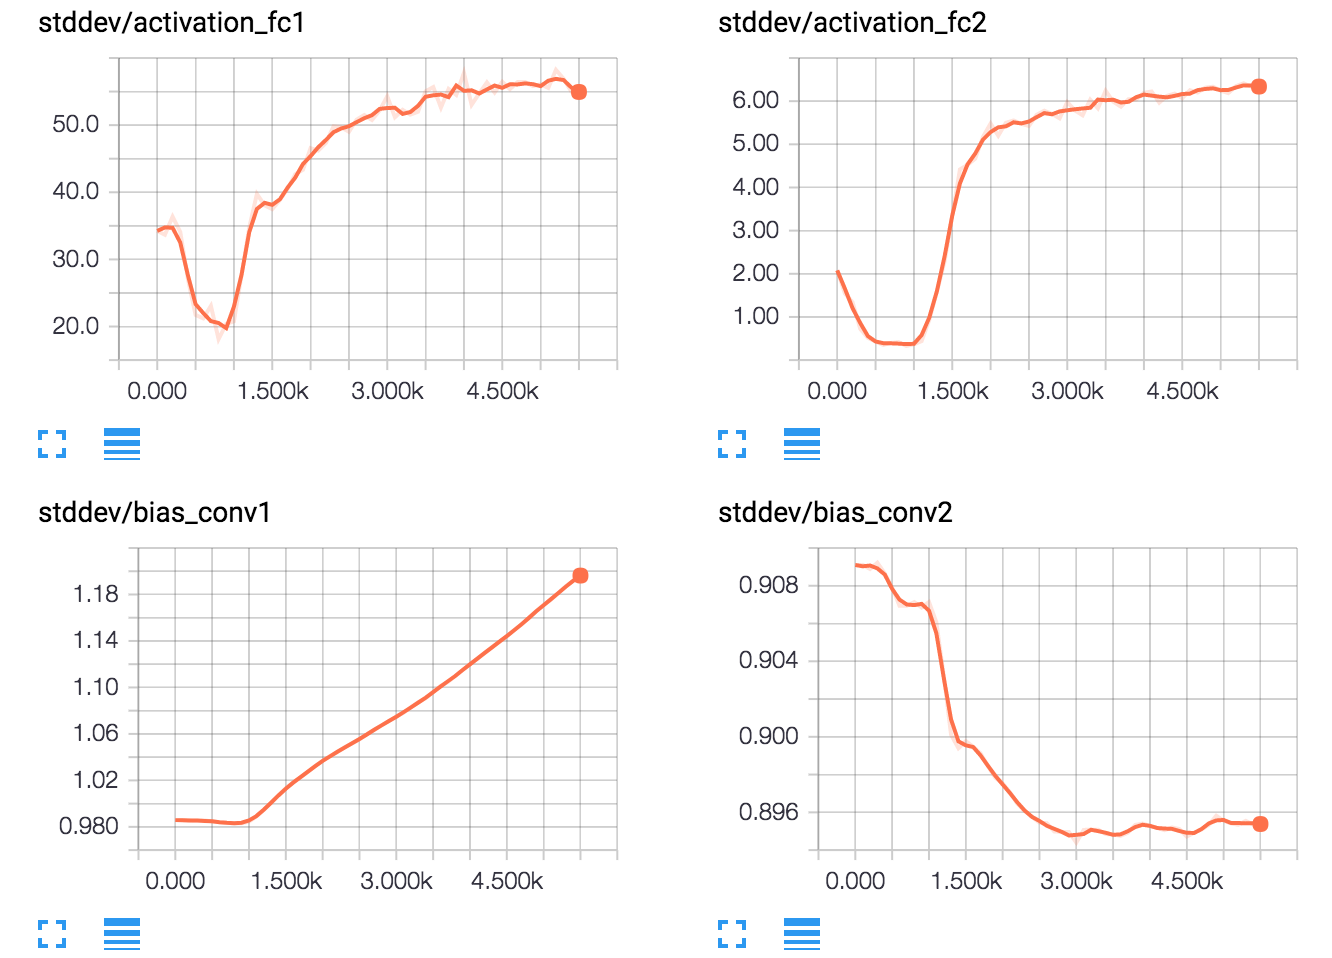
\includegraphics[scale=0.3]{st2.png}
\end{figure}
\begin{figure}[H]
  \caption{center}
  \centering
    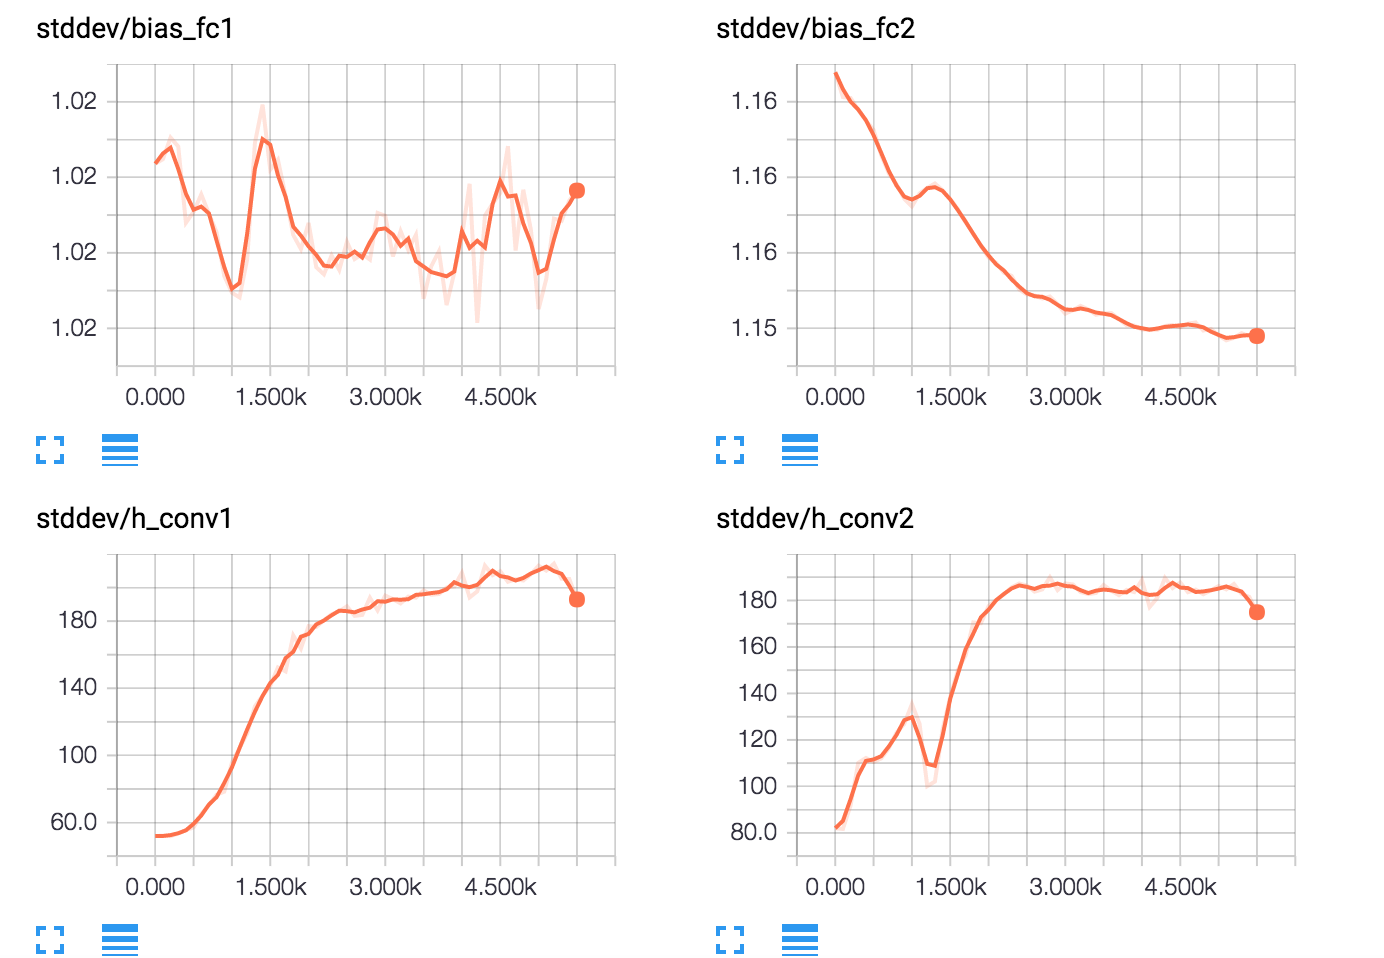
\includegraphics[scale=0.3]{st3.png}
\end{figure}
\begin{figure}[H]
  \caption{center}
  \centering
    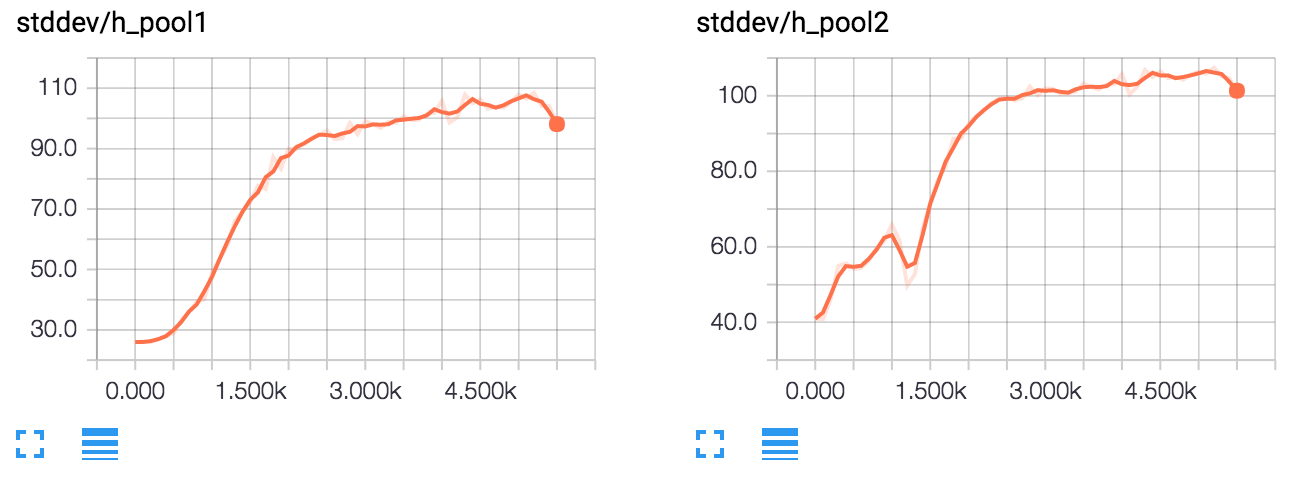
\includegraphics[scale=0.3]{st4.png}
\end{figure}
I used relu function, RMSPropOptimizer. After 5500 training, the validation accuracy is 0.98, which is better than sigmond funciton. Usually relu has better performance than sigmond. 
The tanh function has final validation accuracy of 0.985. It also has good performance. Since the amount of pictures is large, I didn't put them here. 

			\end{document}

